\documentclass{beamer}
%for handout use the follwing
%\documentclass[handout]{beamer}

%\usepackage{beamerthemeshadow}
\usetheme{Warsaw}
%\usepackage{bbm}
%\usepackage{mathptm}
\usepackage{xspace}
\usepackage{tikz} 	% to overlay grpahics
%\usepackage[export]{adjustbox}		% for left/ right align of graphics
% for citation
%\usepackage{natbib}

% text around a figure
%\usepackage{wrapfig}

% subfloat subfigures
\usepackage[caption=false]{subfig}
% for multirow figures
\usepackage{multirow}

\setbeamertemplate{navigation symbols}{}%remove navigation symbols
%\setbeamertemplate{footline}[frame number]
\addtobeamertemplate{navigation symbols}{}{%
    \usebeamerfont{footline}%
    \usebeamercolor[fg]{footline}%
    \hspace{1em}%
    \insertframenumber/\inserttotalframenumber
}
% \newcommand{\EXACUS}{{\sc Exacus}\xspace}
% \newcommand{\N}{{\mathbb N}}
% \newcommand{\Z}{{\mathbb Z}}
% \newcommand{\Q}{{\mathbb Q}}
% \newcommand{\R}{{\mathbb R}}
% \newcommand{\GCD}{{\em gcd}\xspace}
% \newcommand{\GGT}{{\em ggT}\xspace}

%\titlegraphic{\vspace{-4cm}\hspace*{-9cm}\includegraphics[width=0.3\textwidth]{figures/1_PROFILES_80m_DATA_Symbols_just1OBS_TO-USE.pdf}}

\begin{document}

\title[TURBO2]{TURBO2: A MATLAB simulation to study the effects of bioturbation on paleoceanographic time series
} % \newline \newline \small{OR: Rotten eggs and car tyres in the ocean}}  
%\author[Dominik H\"ulse, University of California Riverside]{Dominik H\"ulse}


\date{16. Mai 2018\\
Riverside - lab meeting
}

%\frame{\titlepage} 

\begin{frame}
 \titlepage
\end{frame}



\begin{frame}
\frametitle{Sediment mixing/bioturbation in TURBO2}
\begin{columns}
\begin{column}{0.4\textwidth}
{\scriptsize
- Simulates the effect of bioturbation on single sediment particles\\[1.5ex]
- Mixed layer model with instantaneous, homogenous mixing \\[1.5ex]
- Mixing depths that vary along the length of the core\\[1.5ex]
- Models signal distortions of isotopic signals from stratigraphic carriers (forams)\\[2.5ex]
}
\end{column}
\begin{column}{0.6\textwidth}
\vspace{-0.8cm}
\begin{figure}[hbtp]
\hspace*{-0.8cm}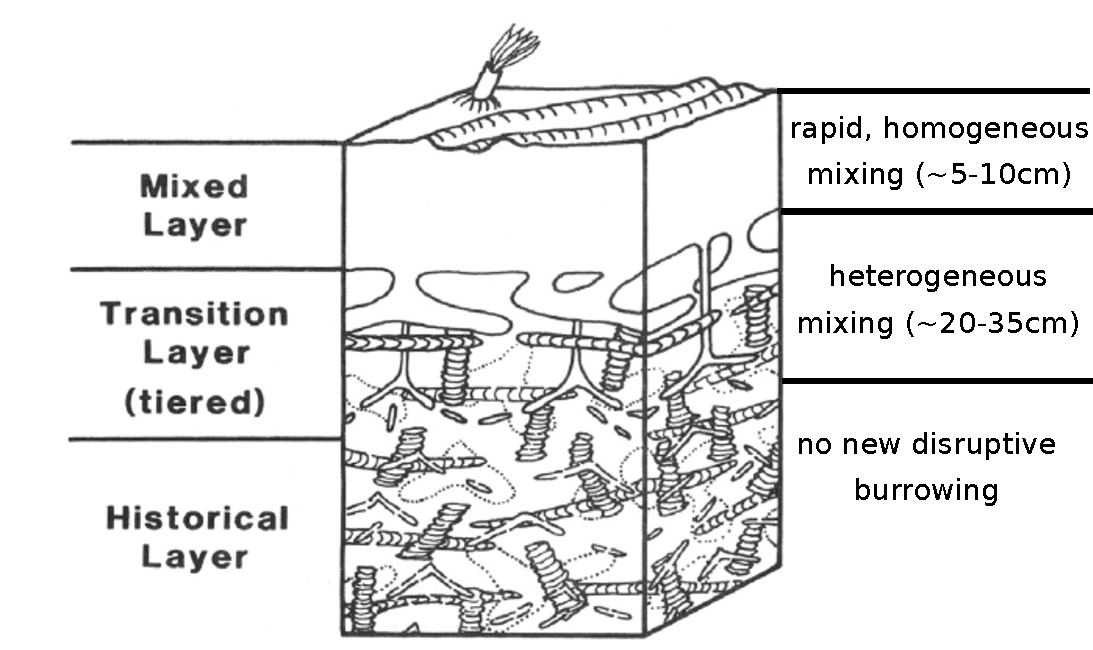
\includegraphics[width=1.1\textwidth]{figures/Sediment_column.pdf}%\caption{Observations from}
\end{figure}
\end{column}
\end{columns}
\end{frame}

\begin{frame}
\frametitle{Experiments}
- Simulate influence of different bioturbation depths on abundance and isotopic signals of 2 species\\[1.5ex]
- real abundance and isotopic signal are covaried (e.g. impulse- or stepchange for both signals)\\[1.5ex]
- $\sim$500 total particles in each layer\\[1.5ex]
- after mixing, 20 of each foram species are picked in each layer and their isotope values are measured
\end{frame}

\begin{frame}
\frametitle{Example: point event + complete species change}
  \begin{figure}
  \begin{center}
\begin{tikzpicture}
  \node (img1) {\hspace{-0.7cm}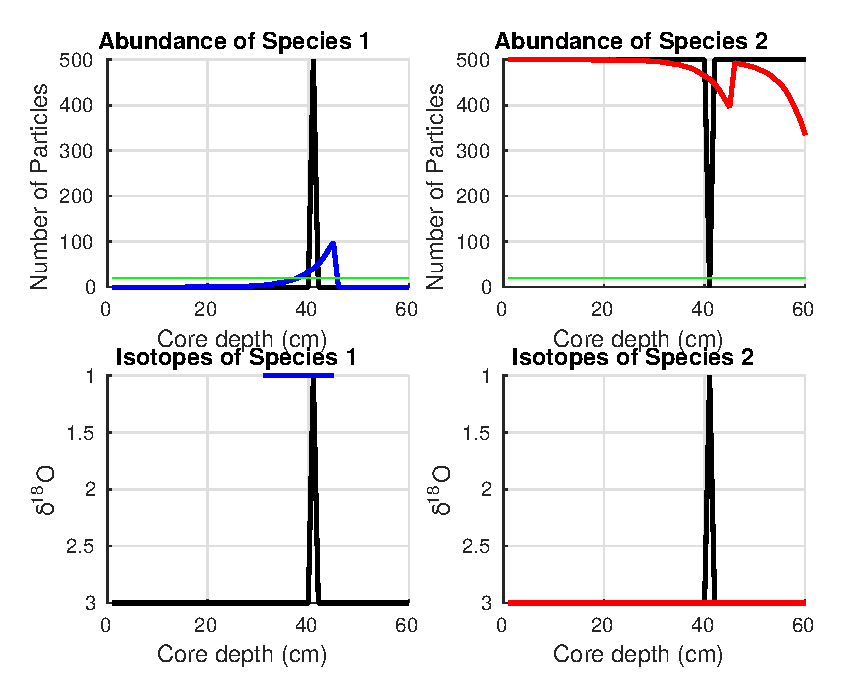
\includegraphics[width=0.9\textwidth]{figures/1point_event_1Exp.pdf}};
  \node (img2) {\hspace{-0.7cm}\includegraphics[width=0.9\textwidth]<2->{figures/1point_event_allExp.pdf}};
\end{tikzpicture}
\end{center}
%\caption[]{\small Modern POC flux data from \cite{lutz_regional_2002}.}
\end{figure}
\end{frame}

\begin{frame}
\frametitle{Example: point event + with background abundance}
\begin{figure}[hbtp]
\hspace*{-0.8cm}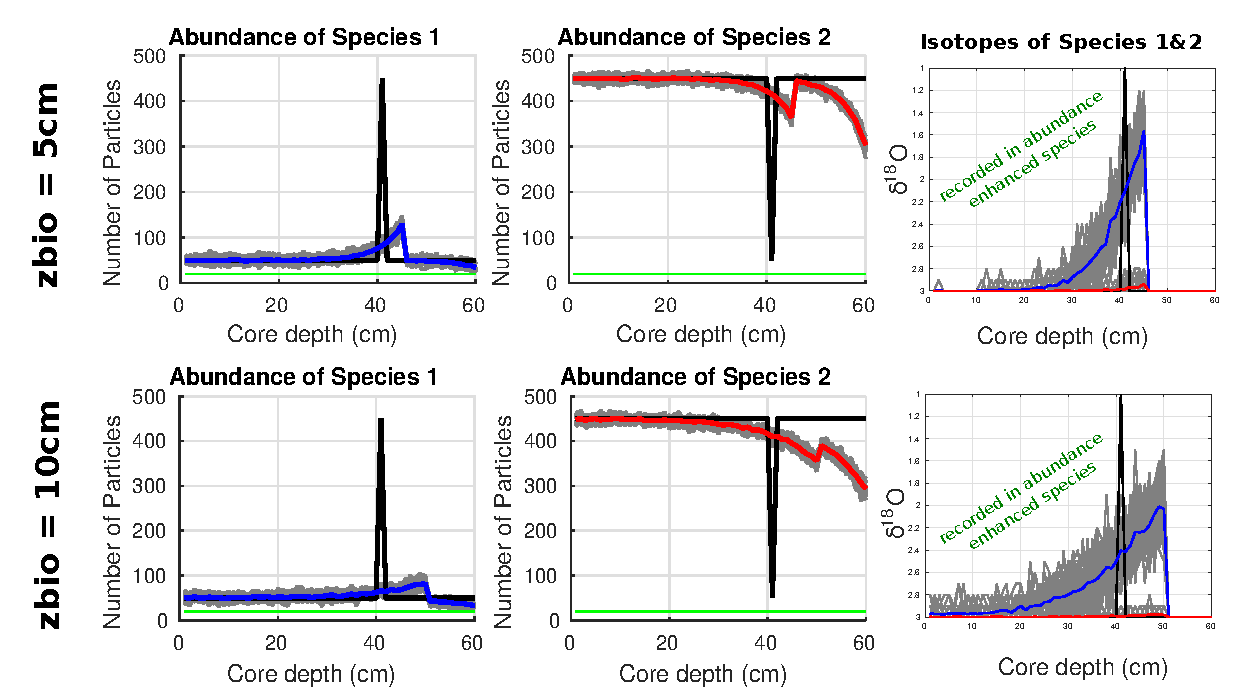
\includegraphics[width=1.1\textwidth]{figures/1point_event_5+10cm_background.pdf}%\caption{Observations from}
\end{figure}
\end{frame}

\begin{frame}
\frametitle{Example: 2 point events + with background abundance}
\begin{figure}[hbtp]
\hspace*{-0.8cm}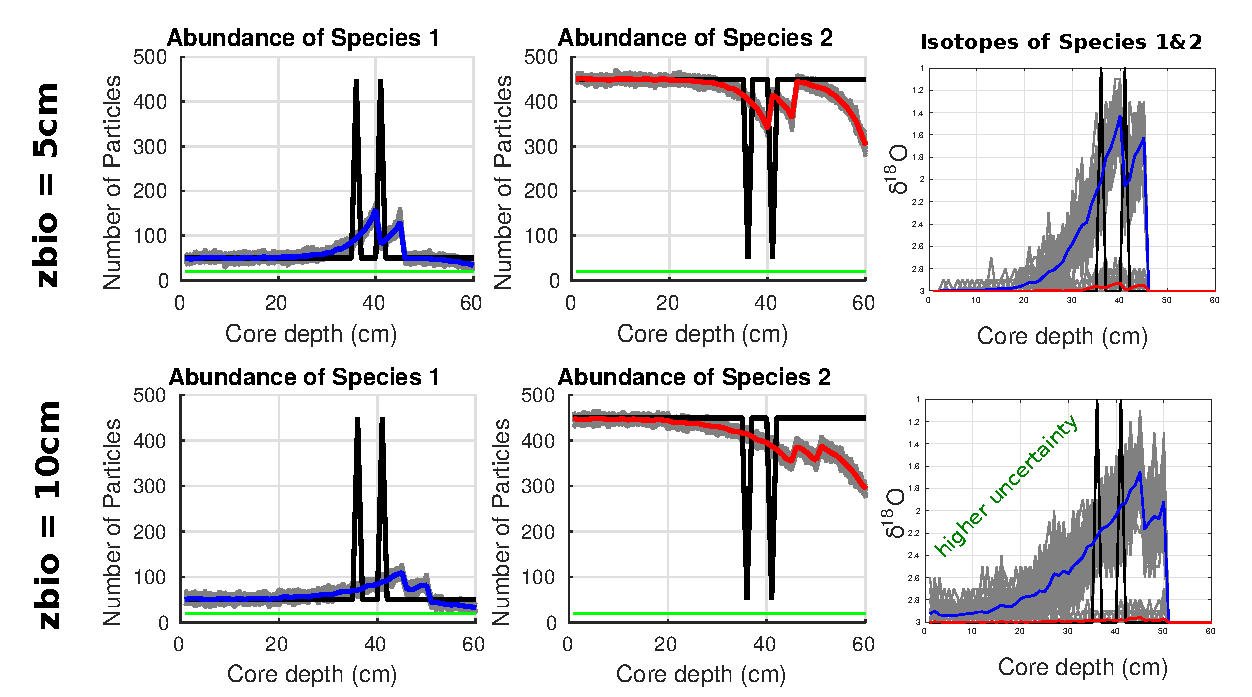
\includegraphics[width=1.1\textwidth]{figures/2point_event_5+10cm_background.pdf}%\caption{Observations from}
\end{figure}
\end{frame}

\begin{frame}
\frametitle{Example: 5 point events + with background abundance}
\begin{figure}[hbtp]
\hspace*{-0.8cm}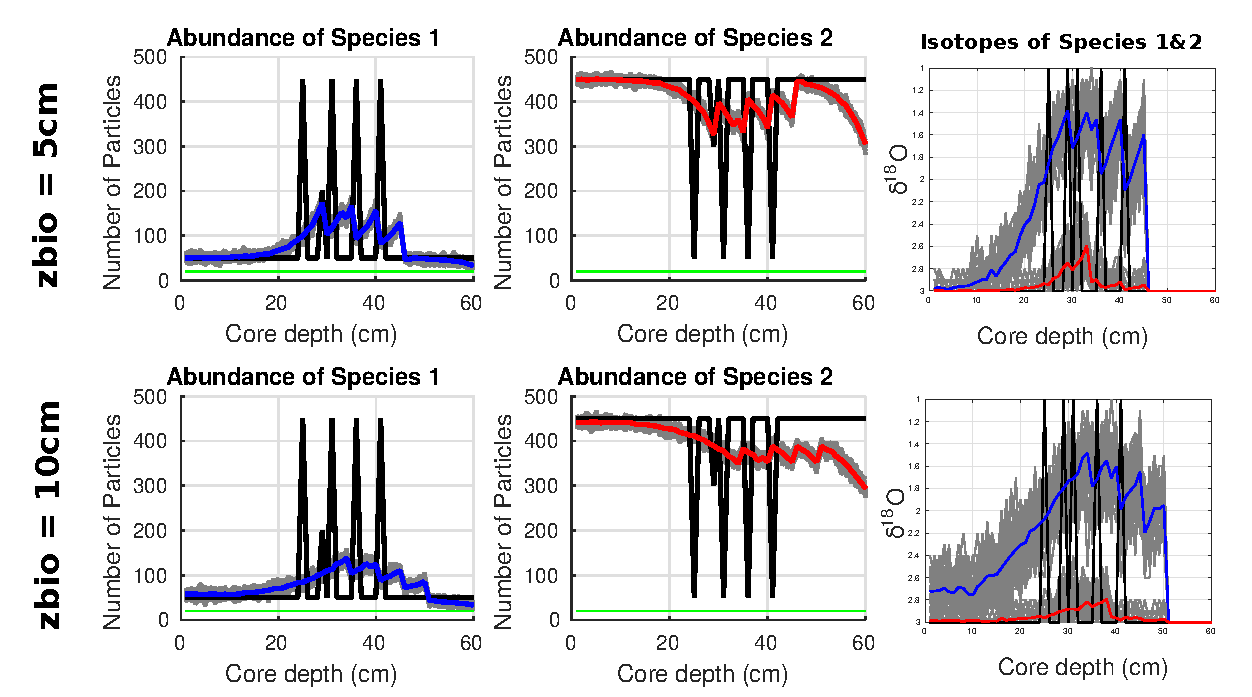
\includegraphics[width=1.1\textwidth]{figures/5point_event_5+10cm_background.pdf}%\caption{Observations from}
\end{figure}
\end{frame}

\begin{frame}
\frametitle{Example: step change + with background abundance}
\begin{figure}[hbtp]
\hspace*{-0.8cm}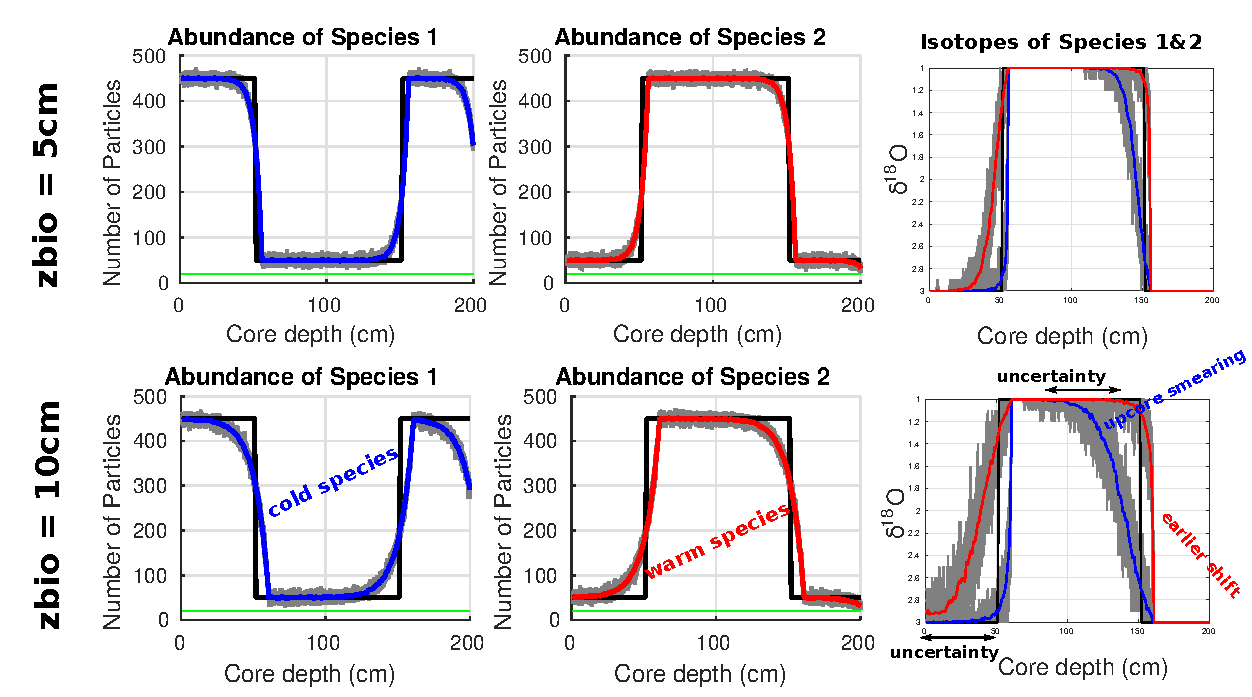
\includegraphics[width=1.1\textwidth]{figures/stepchange2_5+10cm_background.pdf}%\caption{Observations from}
\end{figure}
\end{frame}

\begin{frame}
\frametitle{Example: gradual change + with background abundance}
\begin{figure}[hbtp]
\hspace*{-0.8cm}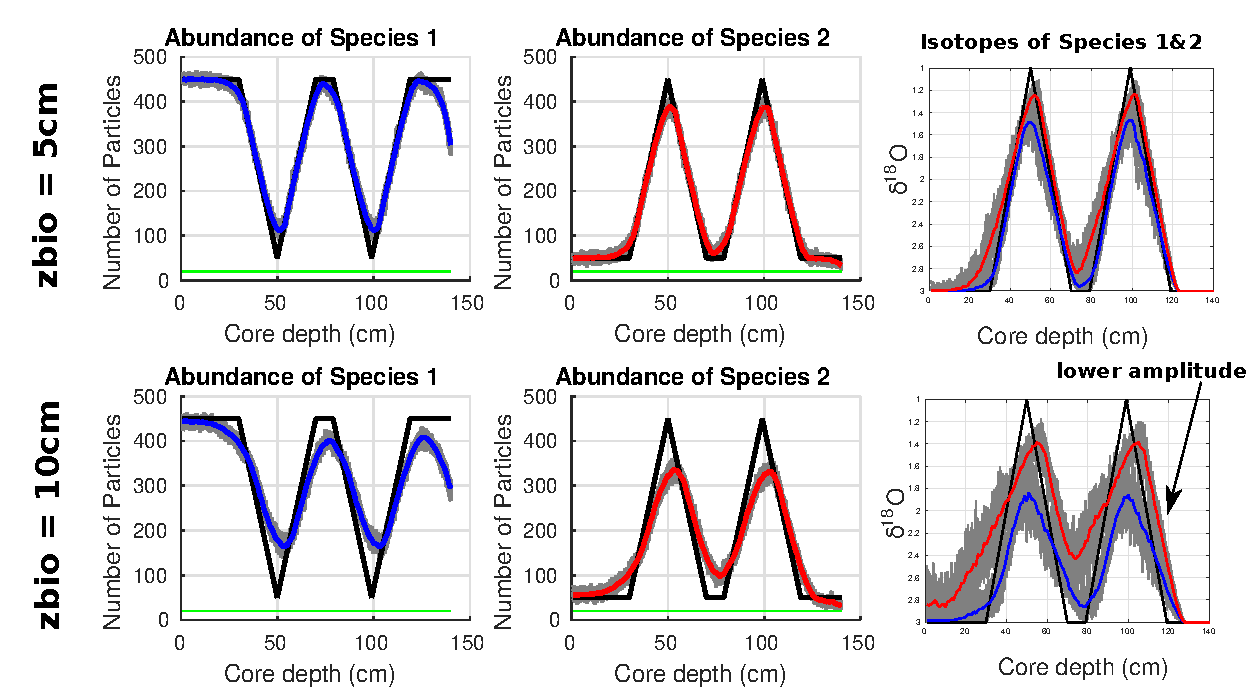
\includegraphics[width=1.1\textwidth]{figures/gradualchange2_5+10cm_background.pdf}%\caption{Observations from}
\end{figure}
\end{frame}

\begin{frame}
\frametitle{Example: 20kyrs cycle}
\begin{figure}[hbtp]
\hspace*{-0.8cm}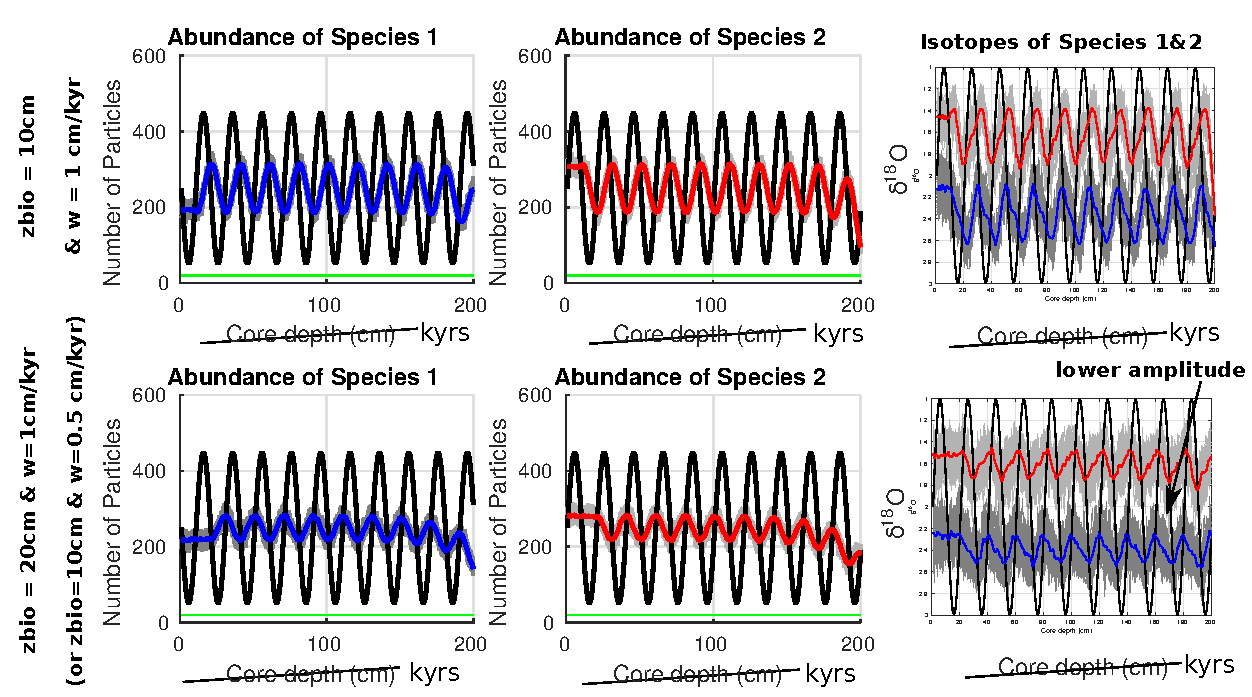
\includegraphics[width=1.1\textwidth]{figures/20kyrcycle_10+20cm_background.pdf}%\caption{Observations from}
\end{figure}
\end{frame}

\begin{frame}
\frametitle{Example: 40kyrs cycle}
\begin{figure}[hbtp]
\hspace*{-0.8cm}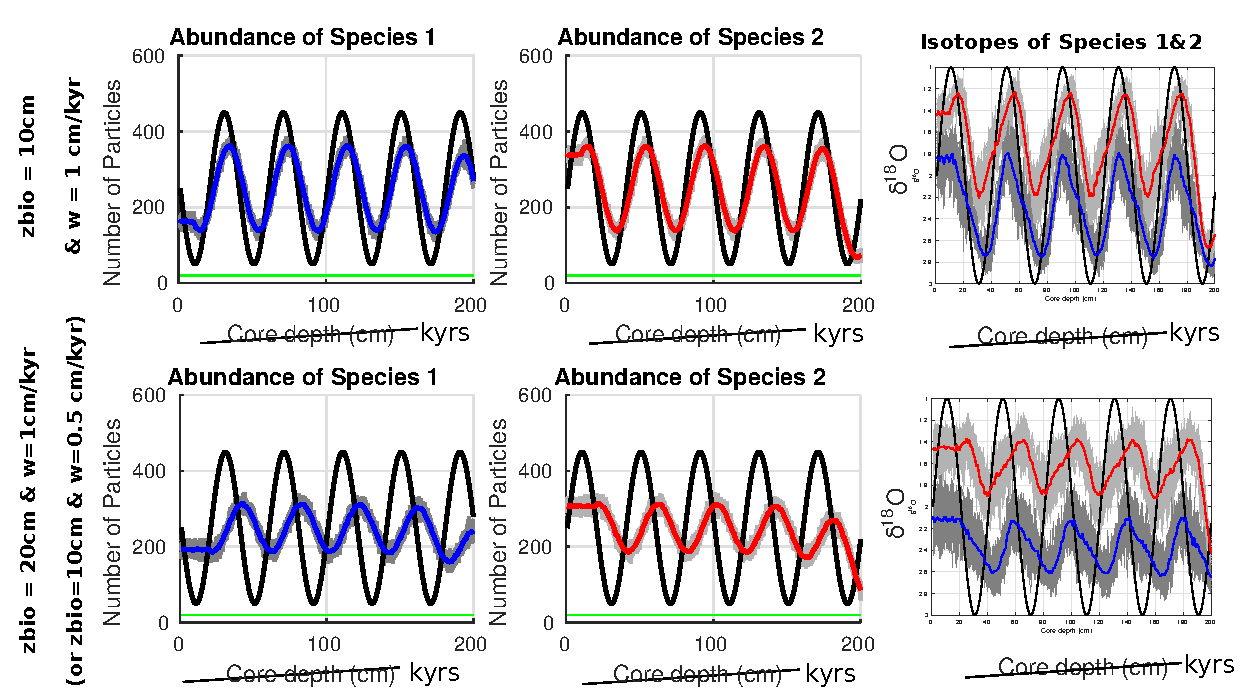
\includegraphics[width=1.1\textwidth]{figures/40kyrcycle_10+20cm_background.pdf}%\caption{Observations from}
\end{figure}
\end{frame}

\begin{frame}
\frametitle{Example: 100kyrs cycle}
\begin{figure}[hbtp]
\hspace*{-0.8cm}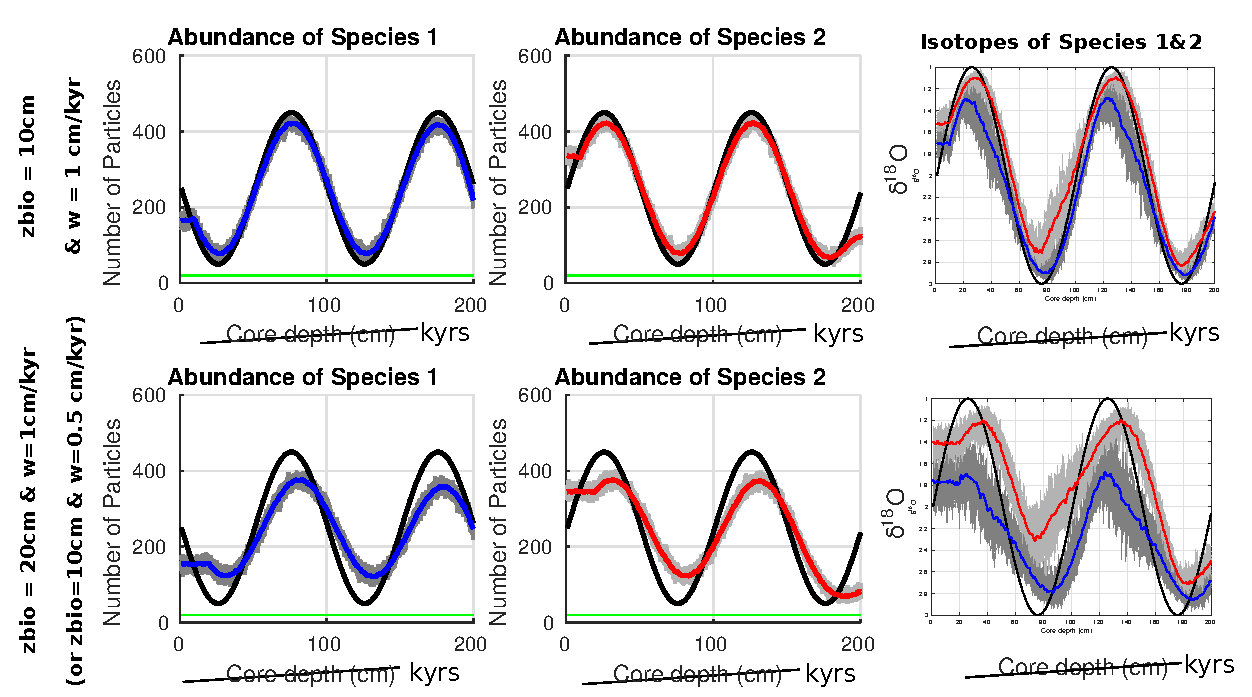
\includegraphics[width=1.1\textwidth]{figures/100kyrcycle_10+20cm_background.pdf}%\caption{Observations from}
\end{figure}
\end{frame}

\begin{frame}
\frametitle{Example: 3 cycles combined}
\begin{figure}[hbtp]
\hspace*{-0.8cm}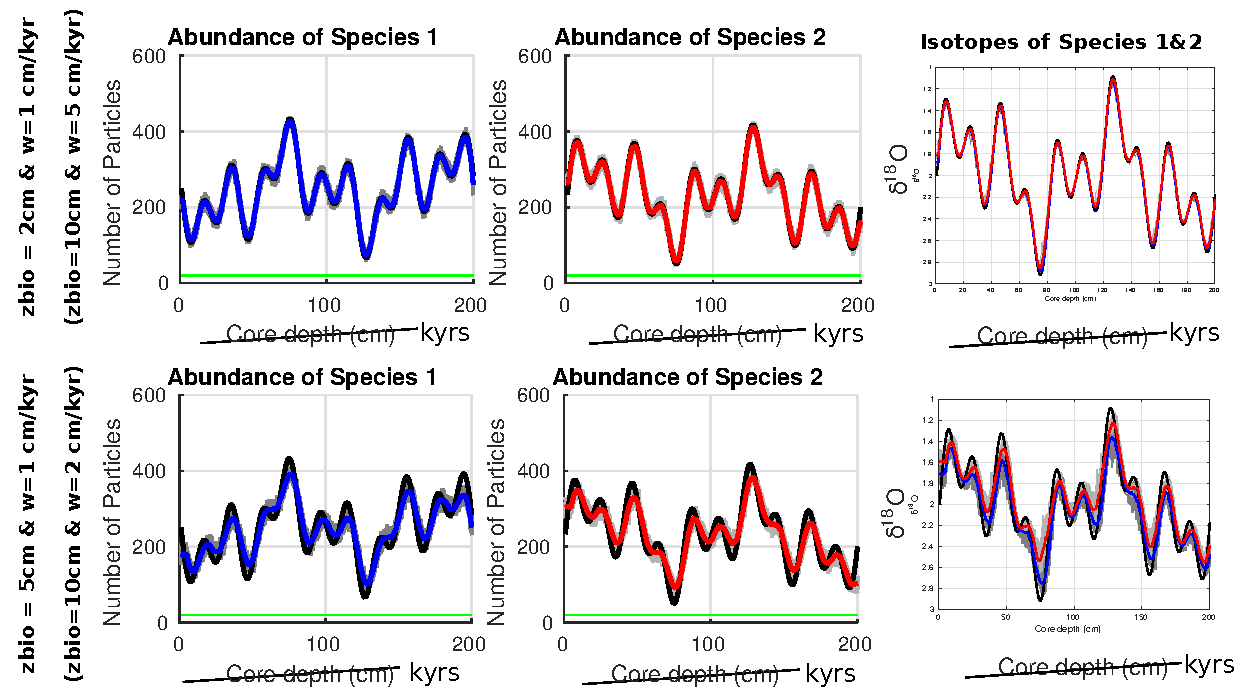
\includegraphics[width=1.1\textwidth]{figures/Allcycles_combined_2+5cm_background.pdf}%\caption{Observations from}
\end{figure}
\end{frame}

\begin{frame}
\frametitle{Example: 3 cycles combined}
\begin{figure}[hbtp]
\hspace*{-0.8cm}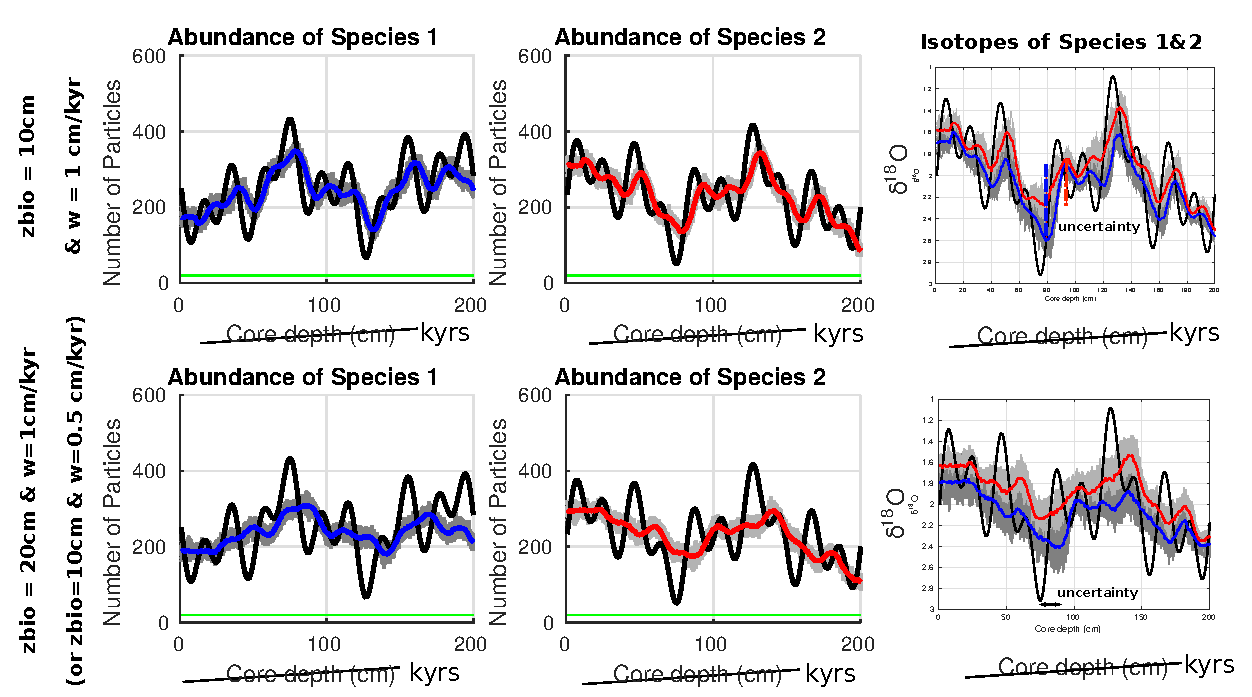
\includegraphics[width=1.1\textwidth]{figures/Allcycles_combined_10+20cm_background.pdf}%\caption{Observations from}
\end{figure}
\end{frame}

\begin{frame}
\frametitle{Example: 3 cycles + point events}
\begin{figure}[hbtp]
\hspace*{-0.8cm}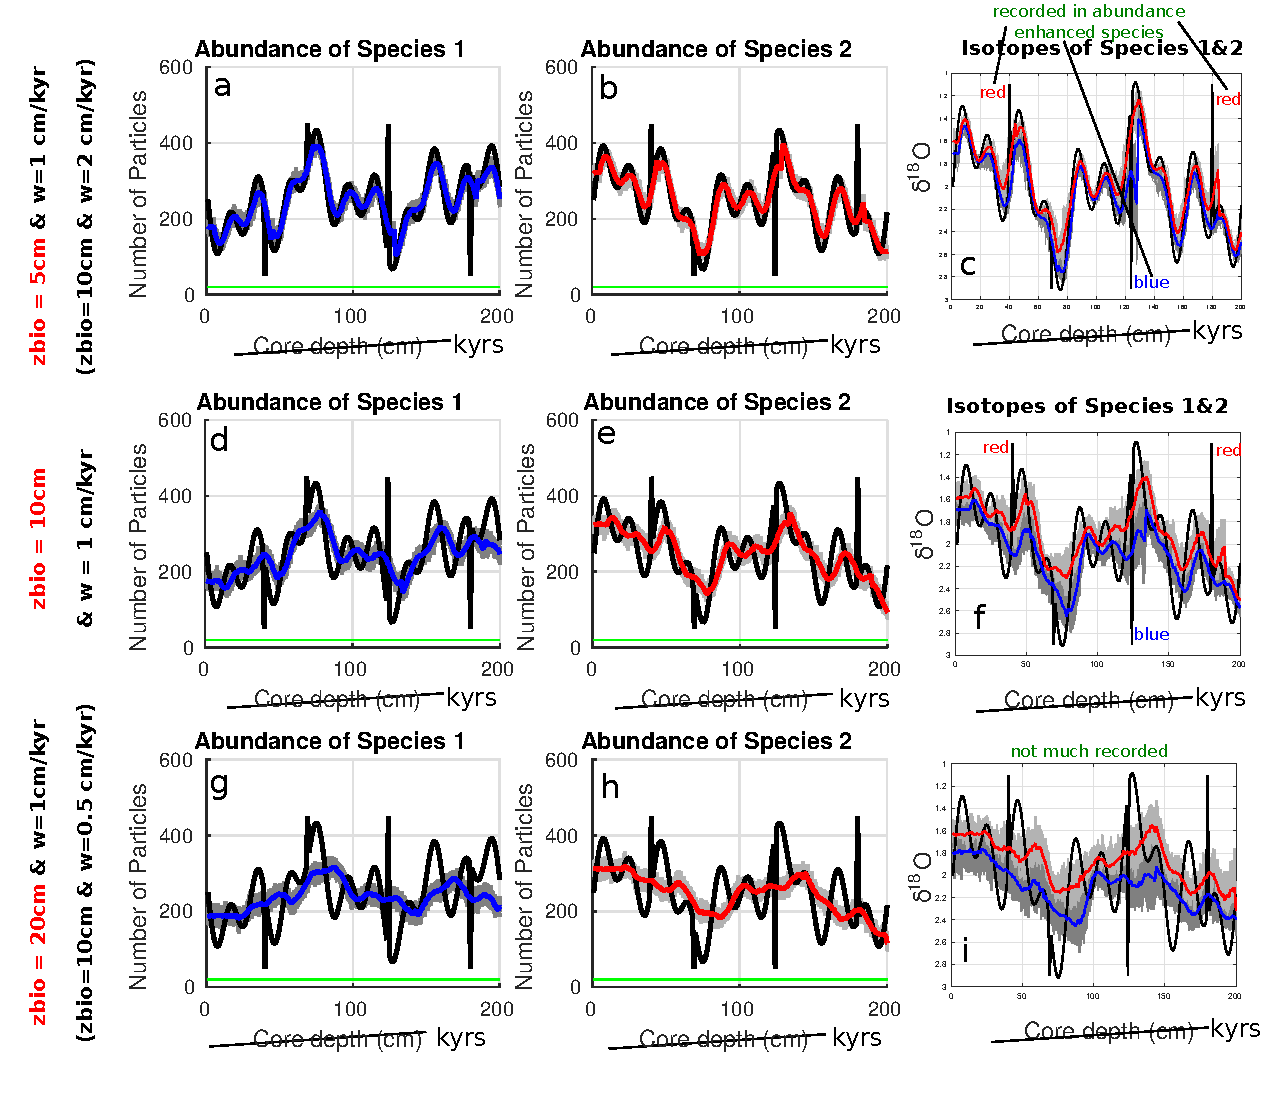
\includegraphics[width=0.9\textwidth]{figures/Allcycles_combined_pointevent_5+10+20cm_background.pdf}%\caption{Observations from}
\end{figure}
\end{frame}

\begin{frame}
\frametitle{Example: 3 cycles + step changes}
\begin{figure}[hbtp]
\hspace*{-0.8cm}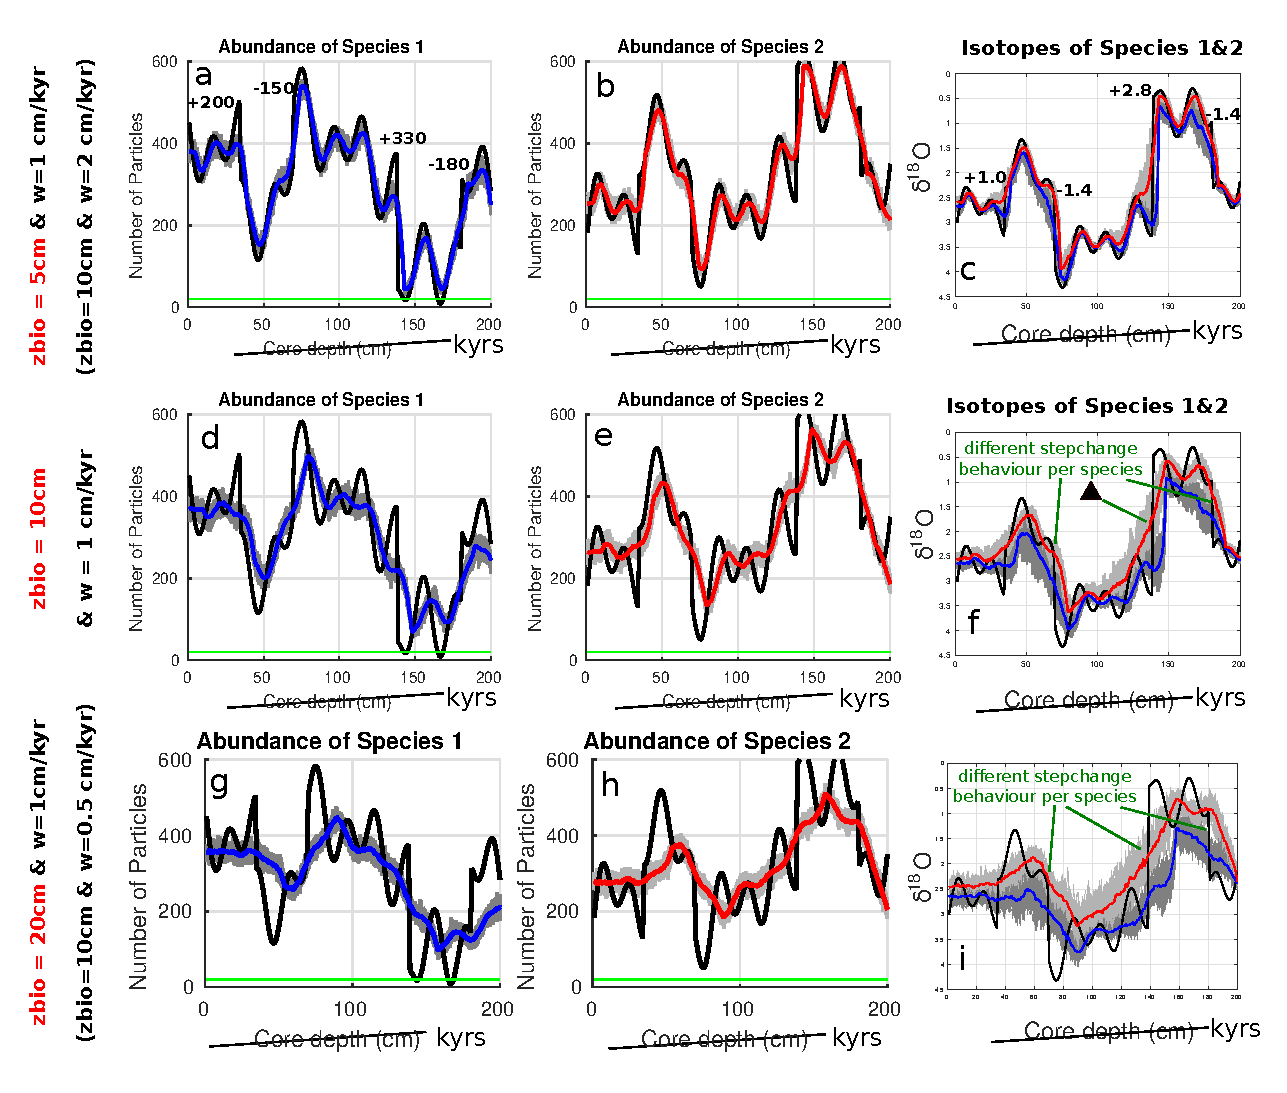
\includegraphics[width=0.9\textwidth]{figures/Allcycles_combined_stepevent_bigger_5+10+20cm_background.pdf}%\caption{Observations from}
\end{figure}
\end{frame}

%% Just change in isotope values
\begin{frame}
\frametitle{Just changes in isotope values}
- just isotopic signal is changed\\[1.5ex]
- $\sim$500 total particles in each layer (350: Species 1; 150: Species 2)\\[1.5ex]
- after mixing, 20 or 5 of each foram species are picked in each layer and their isotope values are measured
\end{frame}

\begin{frame}
\frametitle{Example: point event}
\begin{figure}[hbtp]
\hspace*{-0.8cm}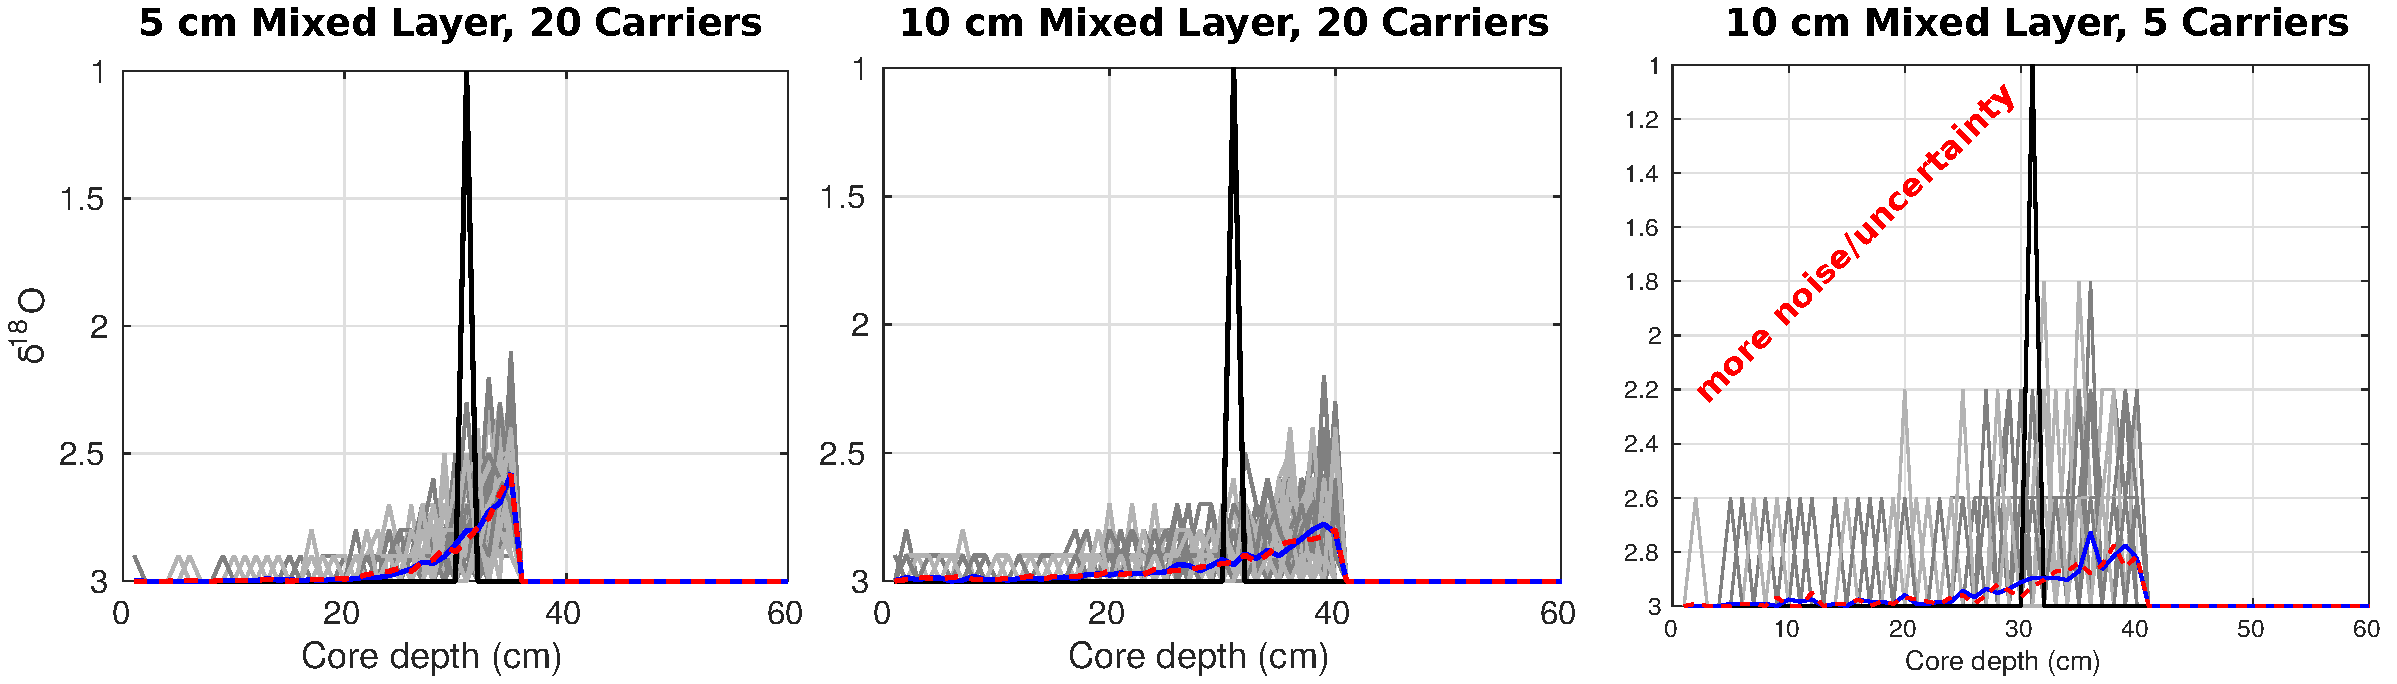
\includegraphics[width=1.1\textwidth]{figures/JustABU_pointevent1.pdf}%\caption{Observations from}
\end{figure}
\end{frame}

\begin{frame}
\frametitle{Example: 2 point events}
\begin{figure}[hbtp]
\hspace*{-0.8cm}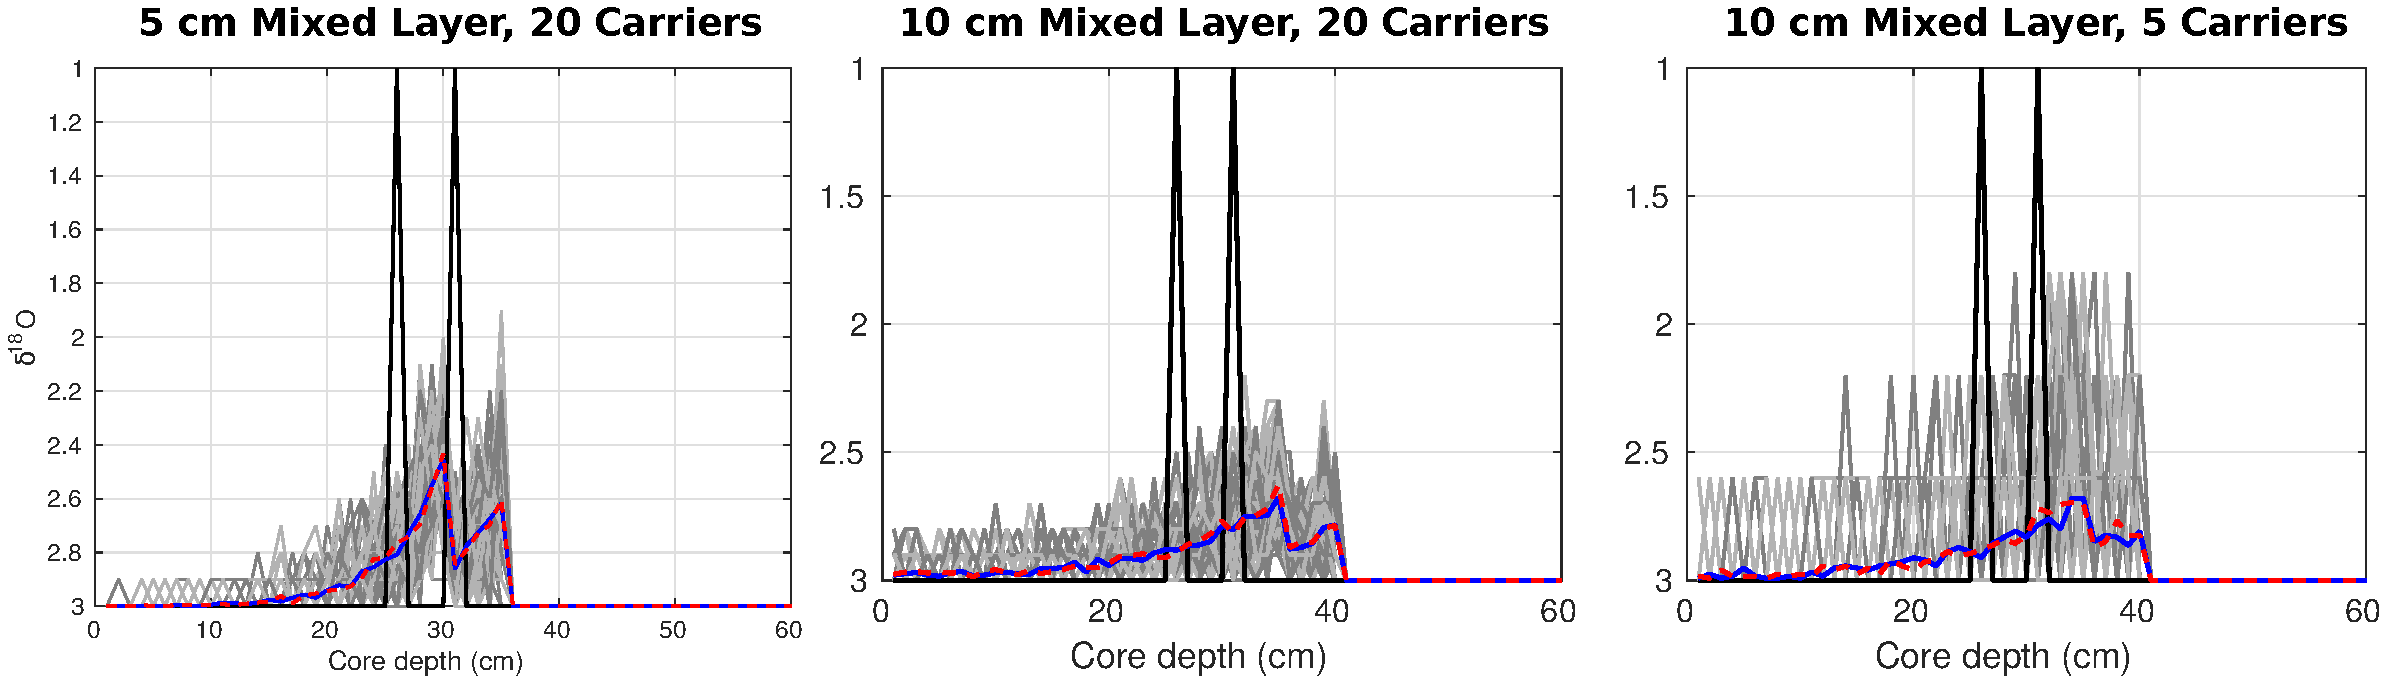
\includegraphics[width=1.1\textwidth]{figures/JustABU_pointevent2.pdf}%\caption{Observations from}
\end{figure}
\end{frame}

\begin{frame}
\frametitle{Example: 5 point events}
\begin{figure}[hbtp]
\hspace*{-0.8cm}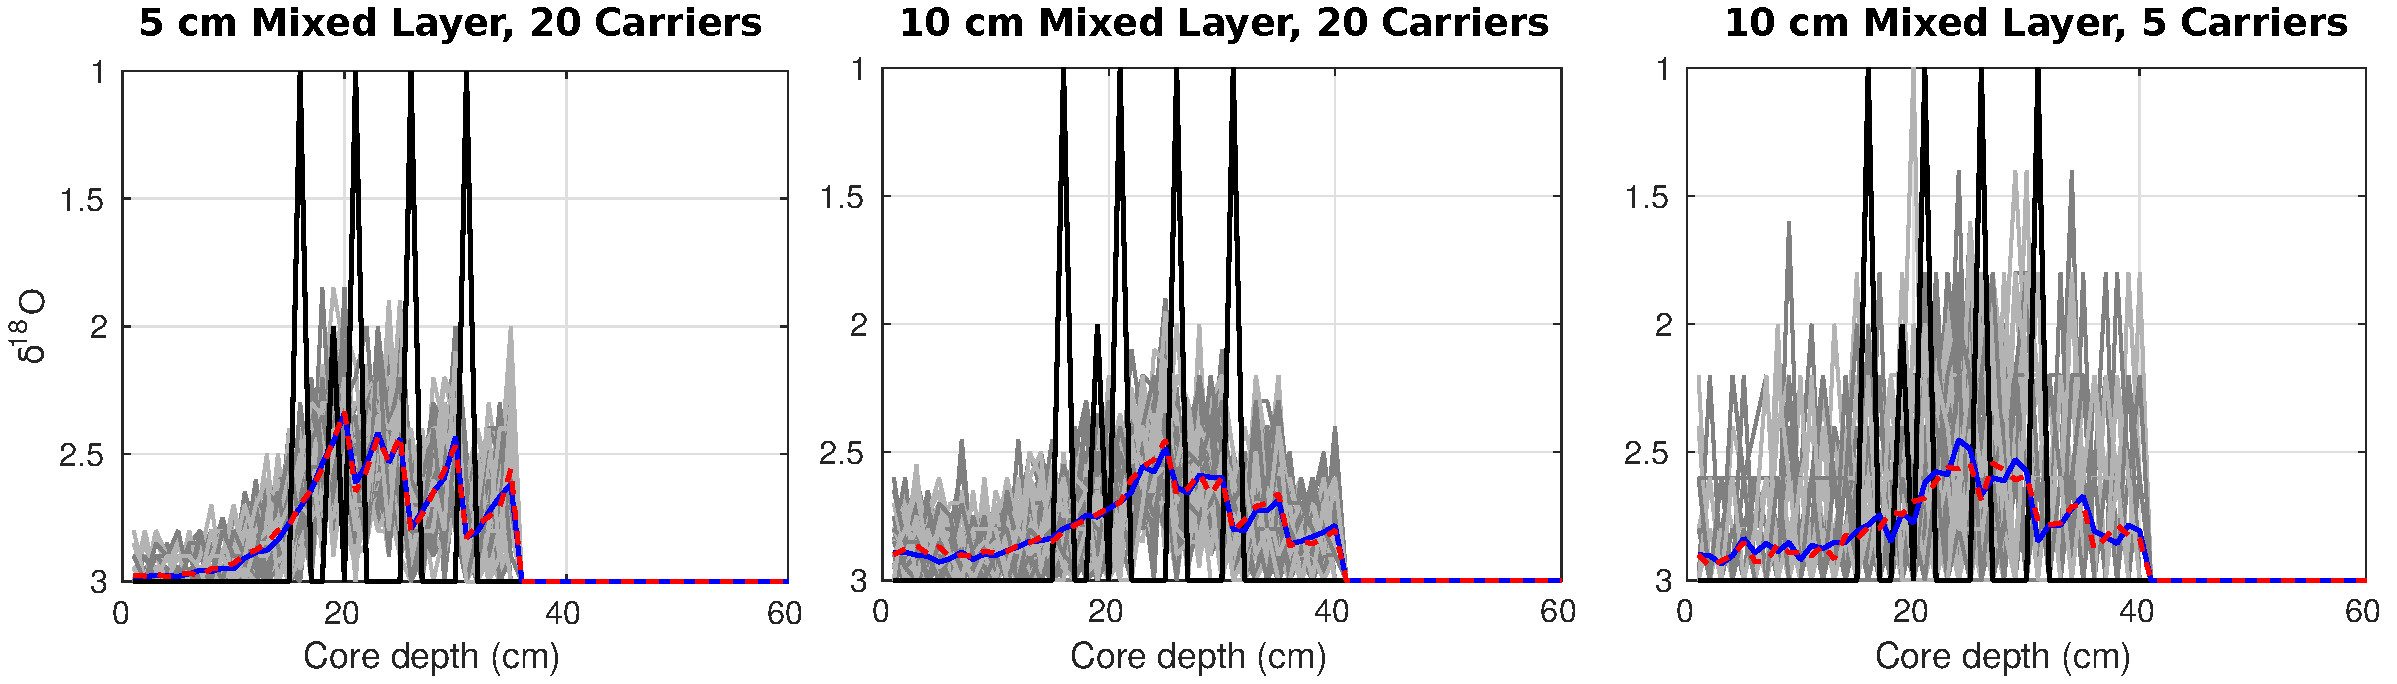
\includegraphics[width=1.1\textwidth]{figures/JustABU_pointevent5.pdf}%\caption{Observations from}
\end{figure}
\end{frame}


\begin{frame}
\frametitle{Example: step change}
\begin{figure}[hbtp]
\hspace*{-0.8cm}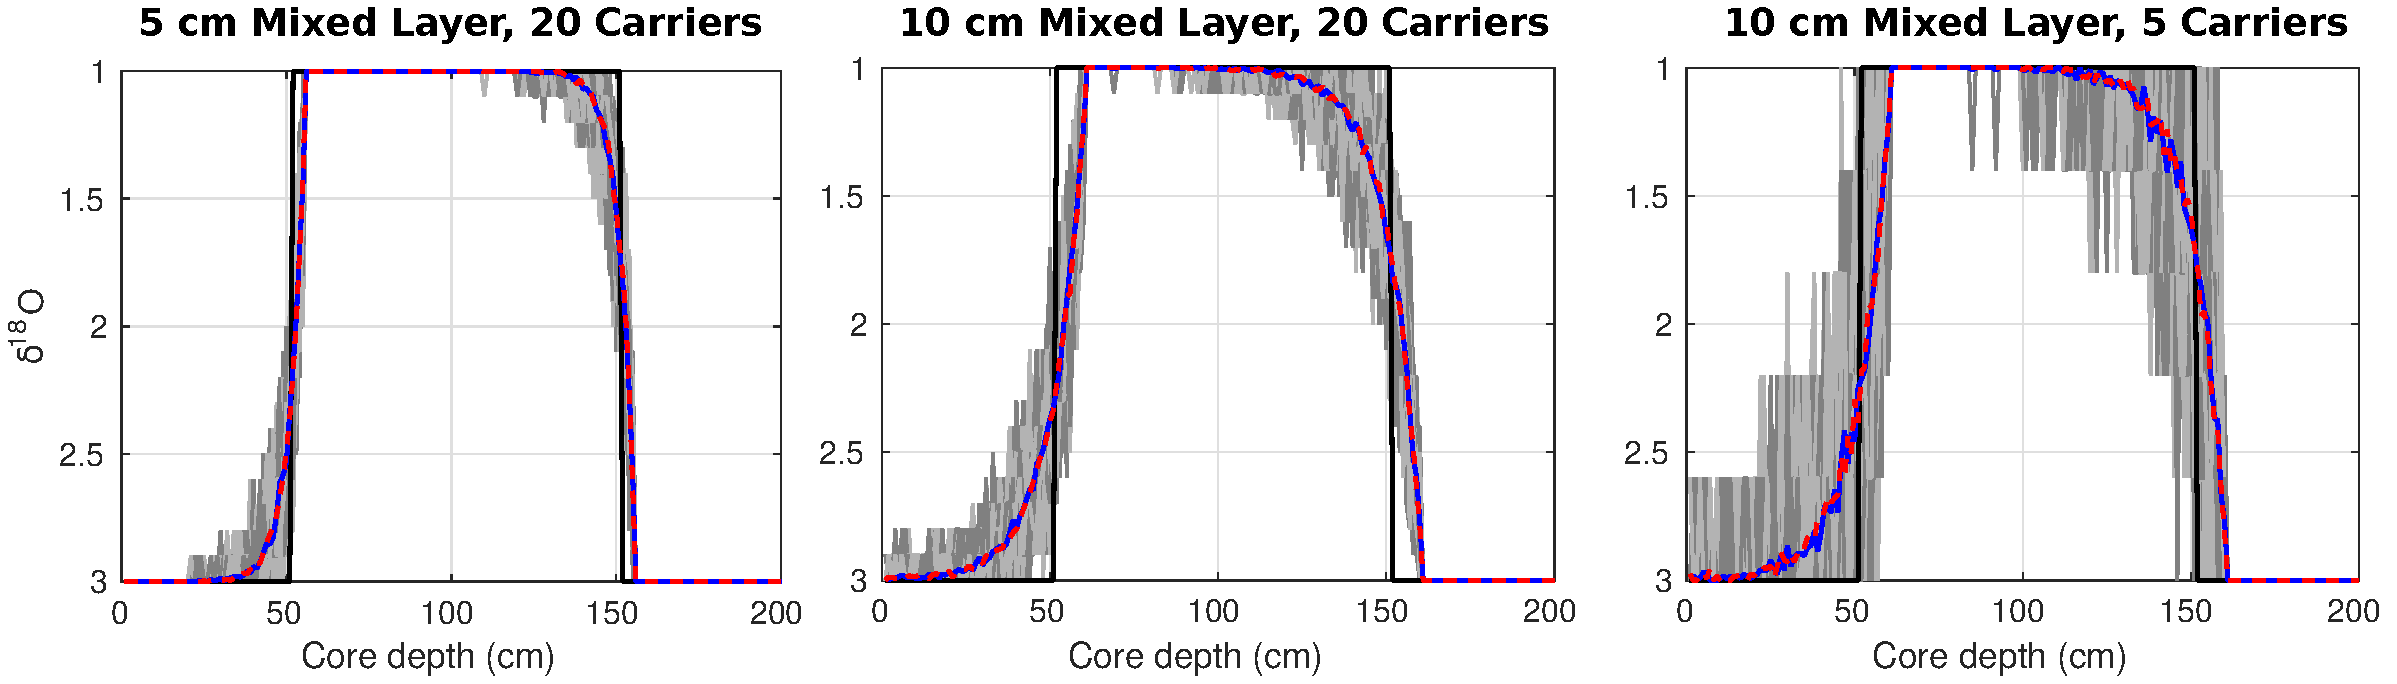
\includegraphics[width=1.1\textwidth]{figures/JustABU_stepchange.pdf}%\caption{Observations from}
\end{figure}
\end{frame}

\begin{frame}
\frametitle{Example: gradual change}
\begin{figure}[hbtp]
\hspace*{-0.8cm}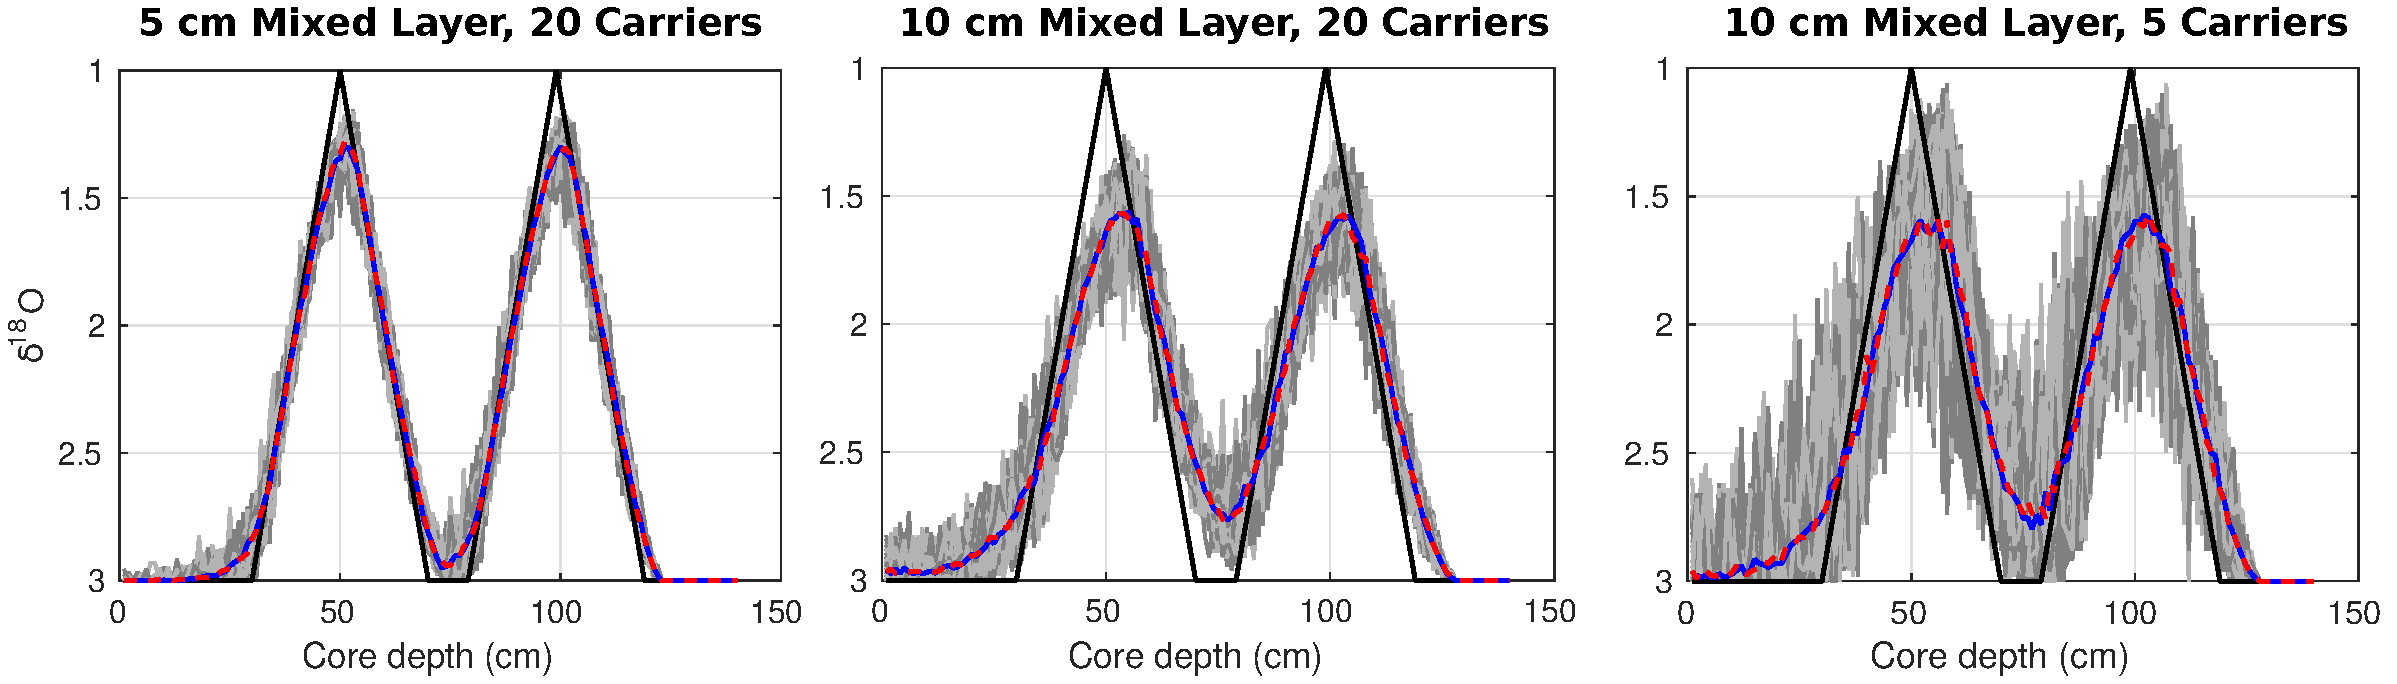
\includegraphics[width=1.1\textwidth]{figures/JustABU_gradualchange.pdf}%\caption{Observations from}
\end{figure}
\end{frame}

\begin{frame}
\frametitle{Example: 20kyrs cycle}
\begin{figure}[hbtp]
\hspace*{-0.8cm}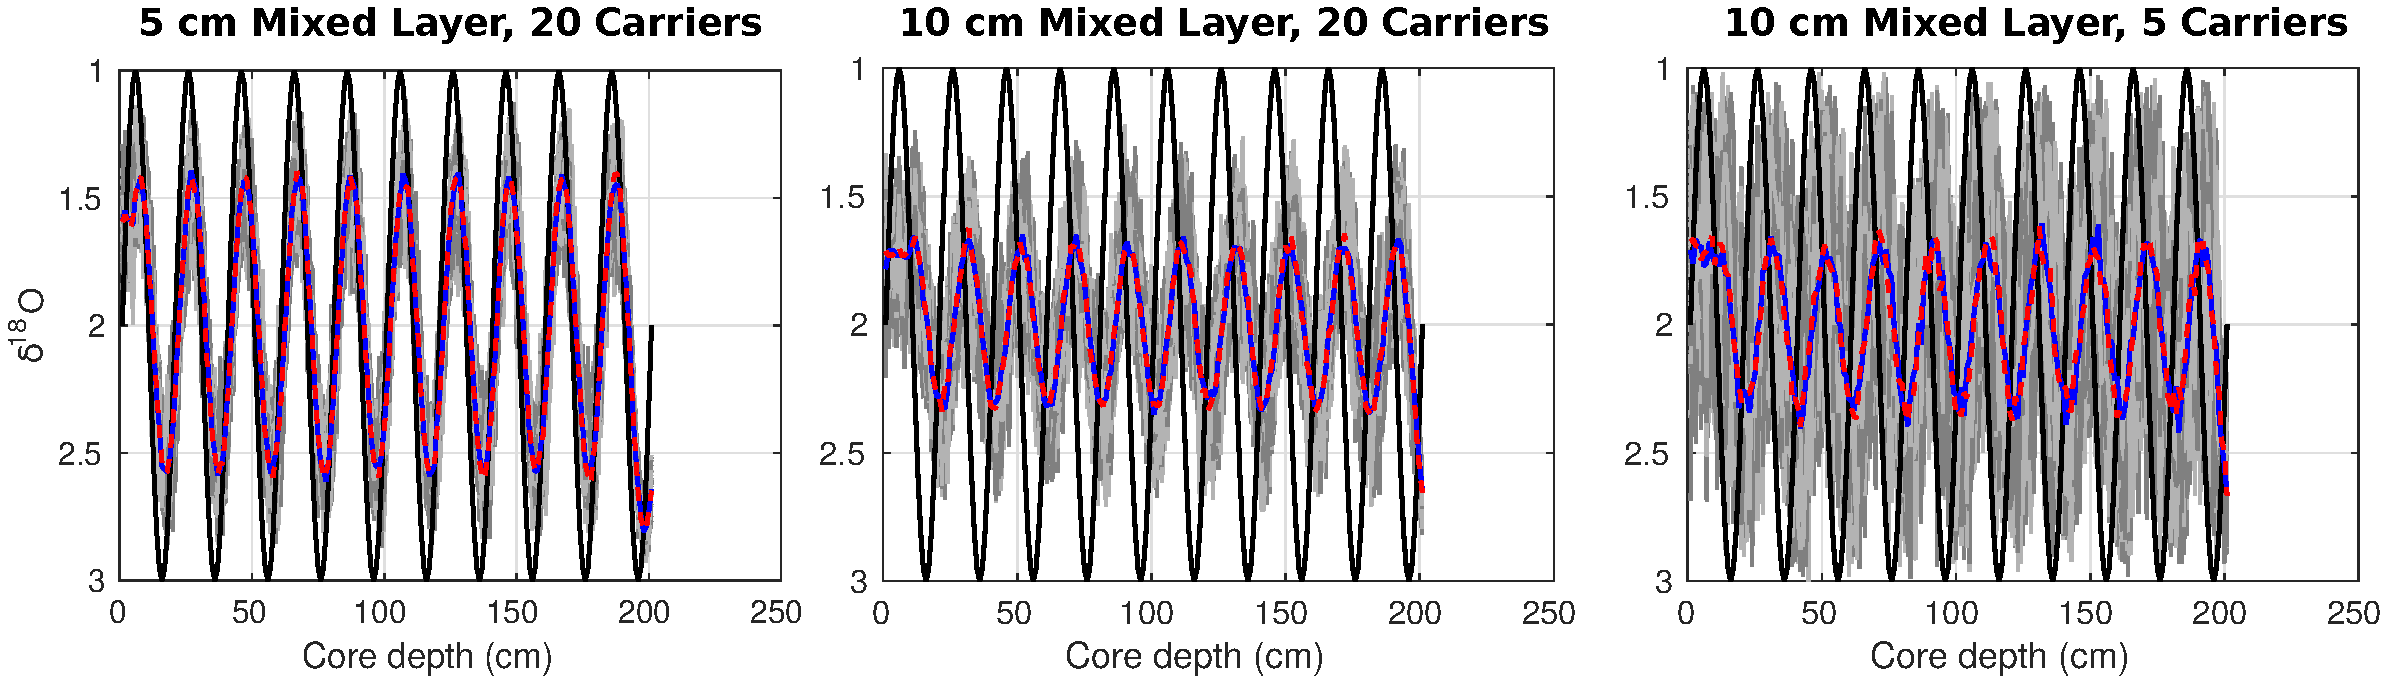
\includegraphics[width=1.1\textwidth]{figures/JustABU_20kyr_cycle.pdf}%\caption{Observations from}
\end{figure}
\end{frame}

\begin{frame}
\frametitle{Example: 40kyrs cycle}
\begin{figure}[hbtp]
\hspace*{-0.8cm}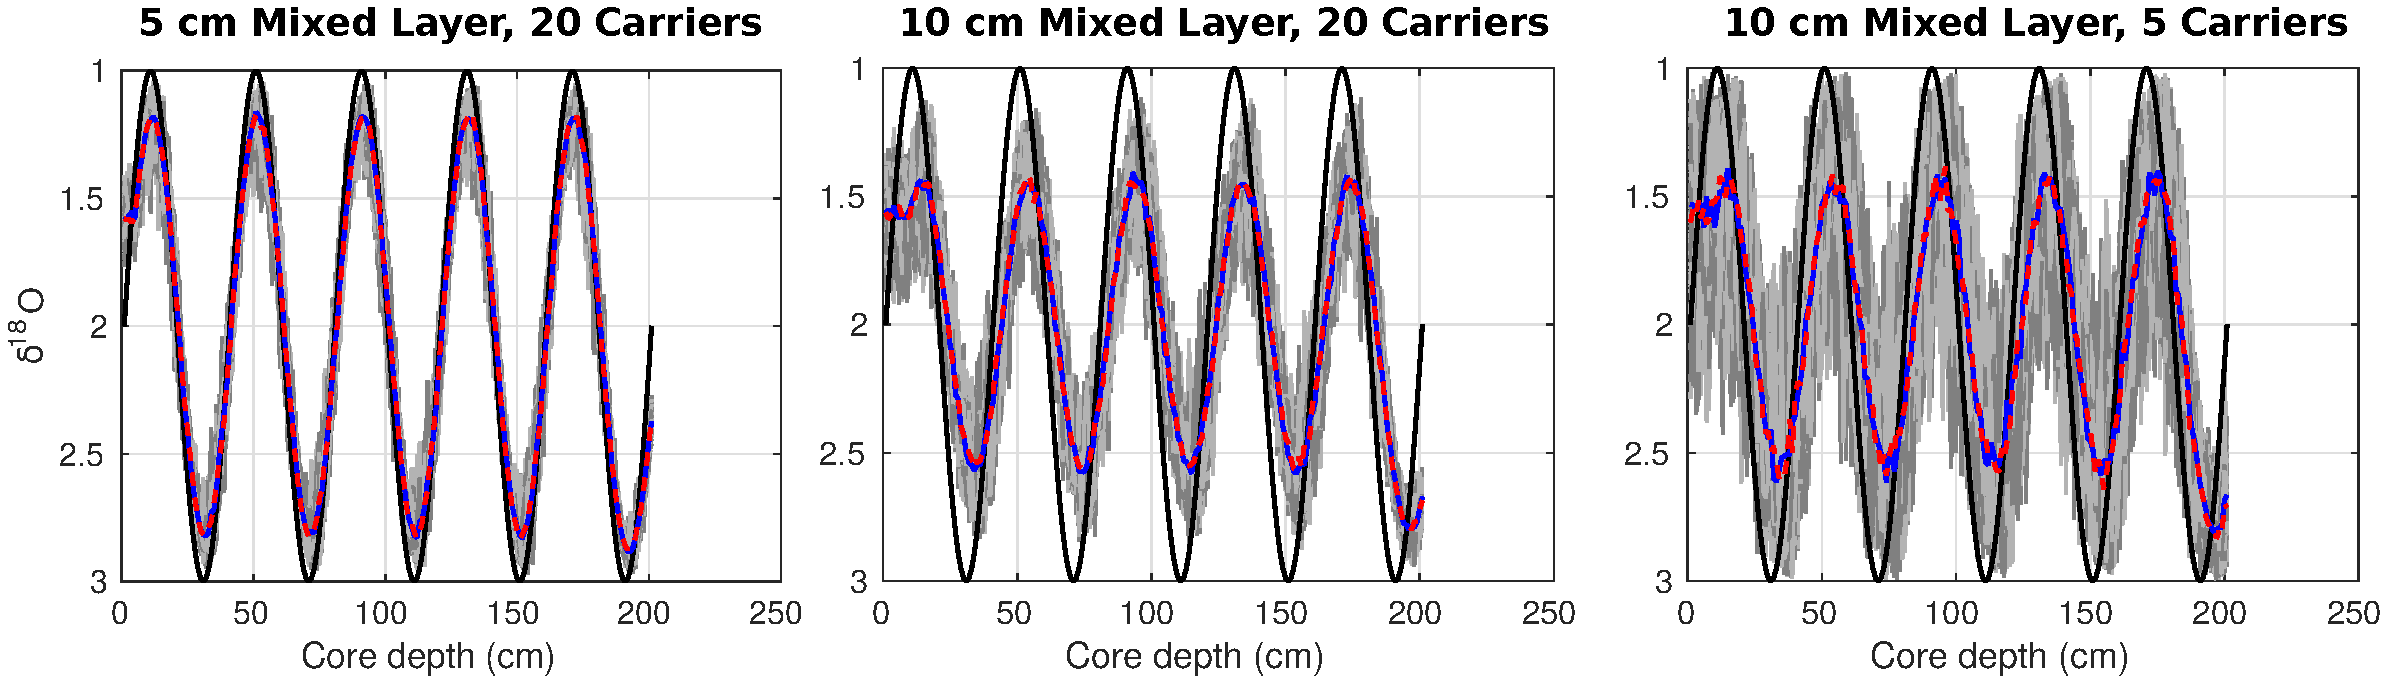
\includegraphics[width=1.1\textwidth]{figures/JustABU_40kyr_cycle.pdf}%\caption{Observations from}
\end{figure}
\end{frame}

\begin{frame}
\frametitle{Example: 100kyrs cycle}
\begin{figure}[hbtp]
\hspace*{-0.8cm}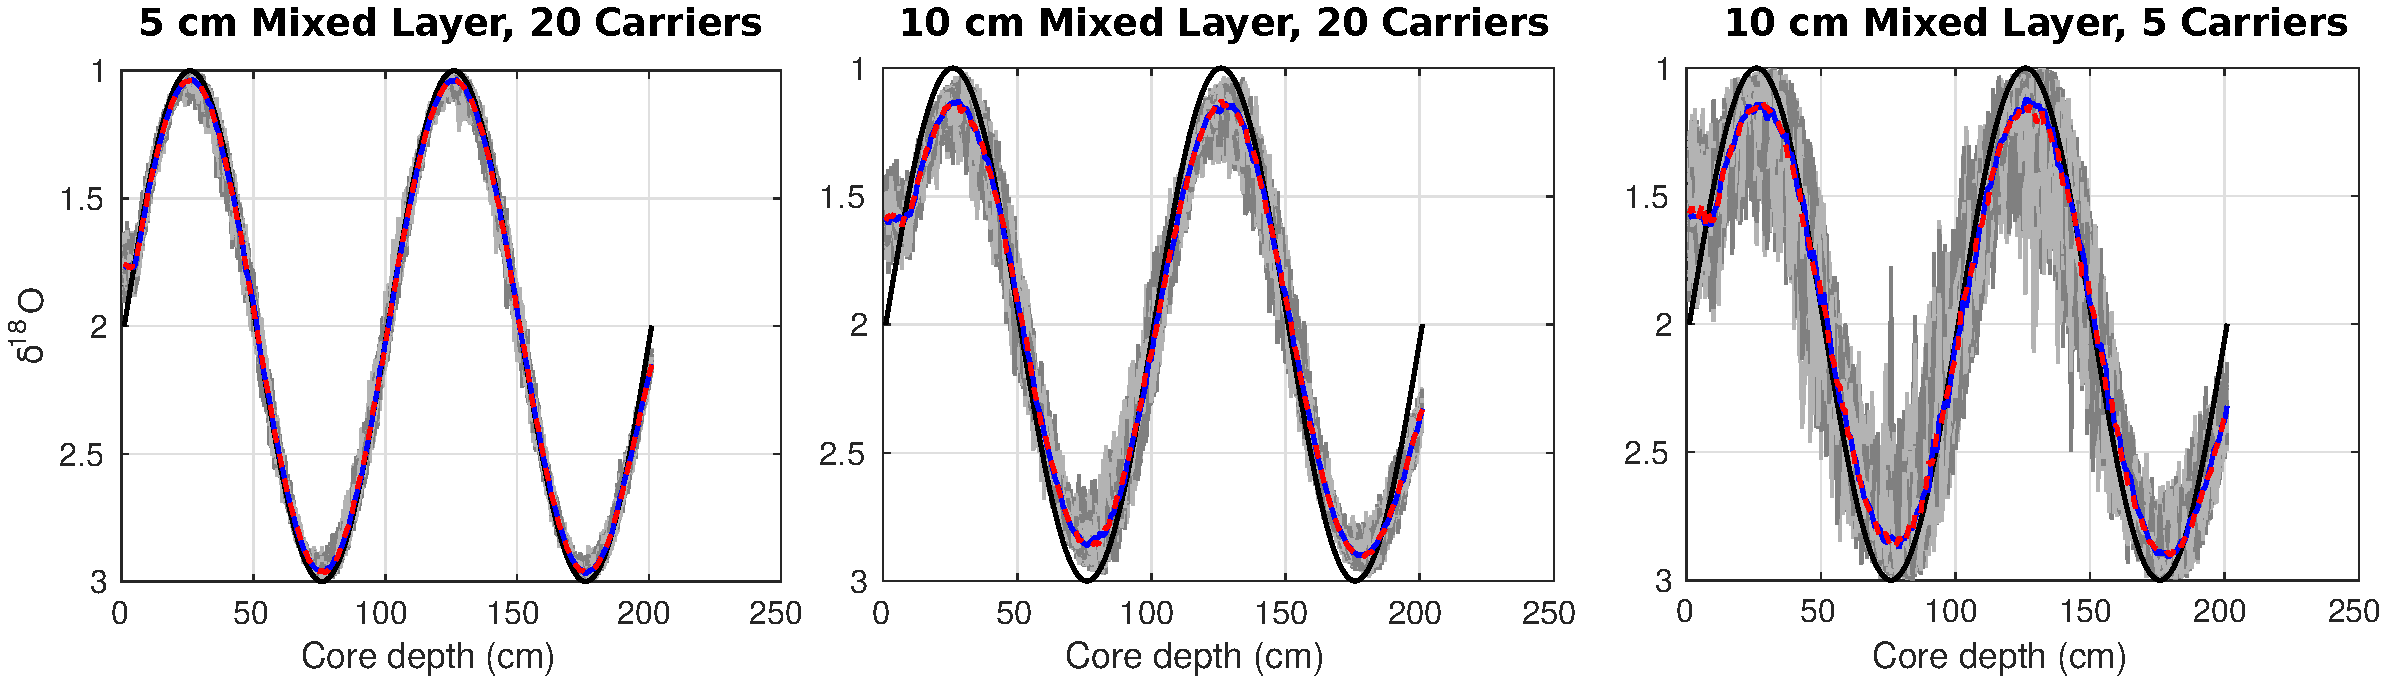
\includegraphics[width=1.1\textwidth]{figures/JustABU_100kyr_cycle.pdf}%\caption{Observations from}
\end{figure}
\end{frame}


\begin{frame}
\frametitle{Example: 3 cycles combined}
\begin{figure}[hbtp]
\hspace*{-0.8cm}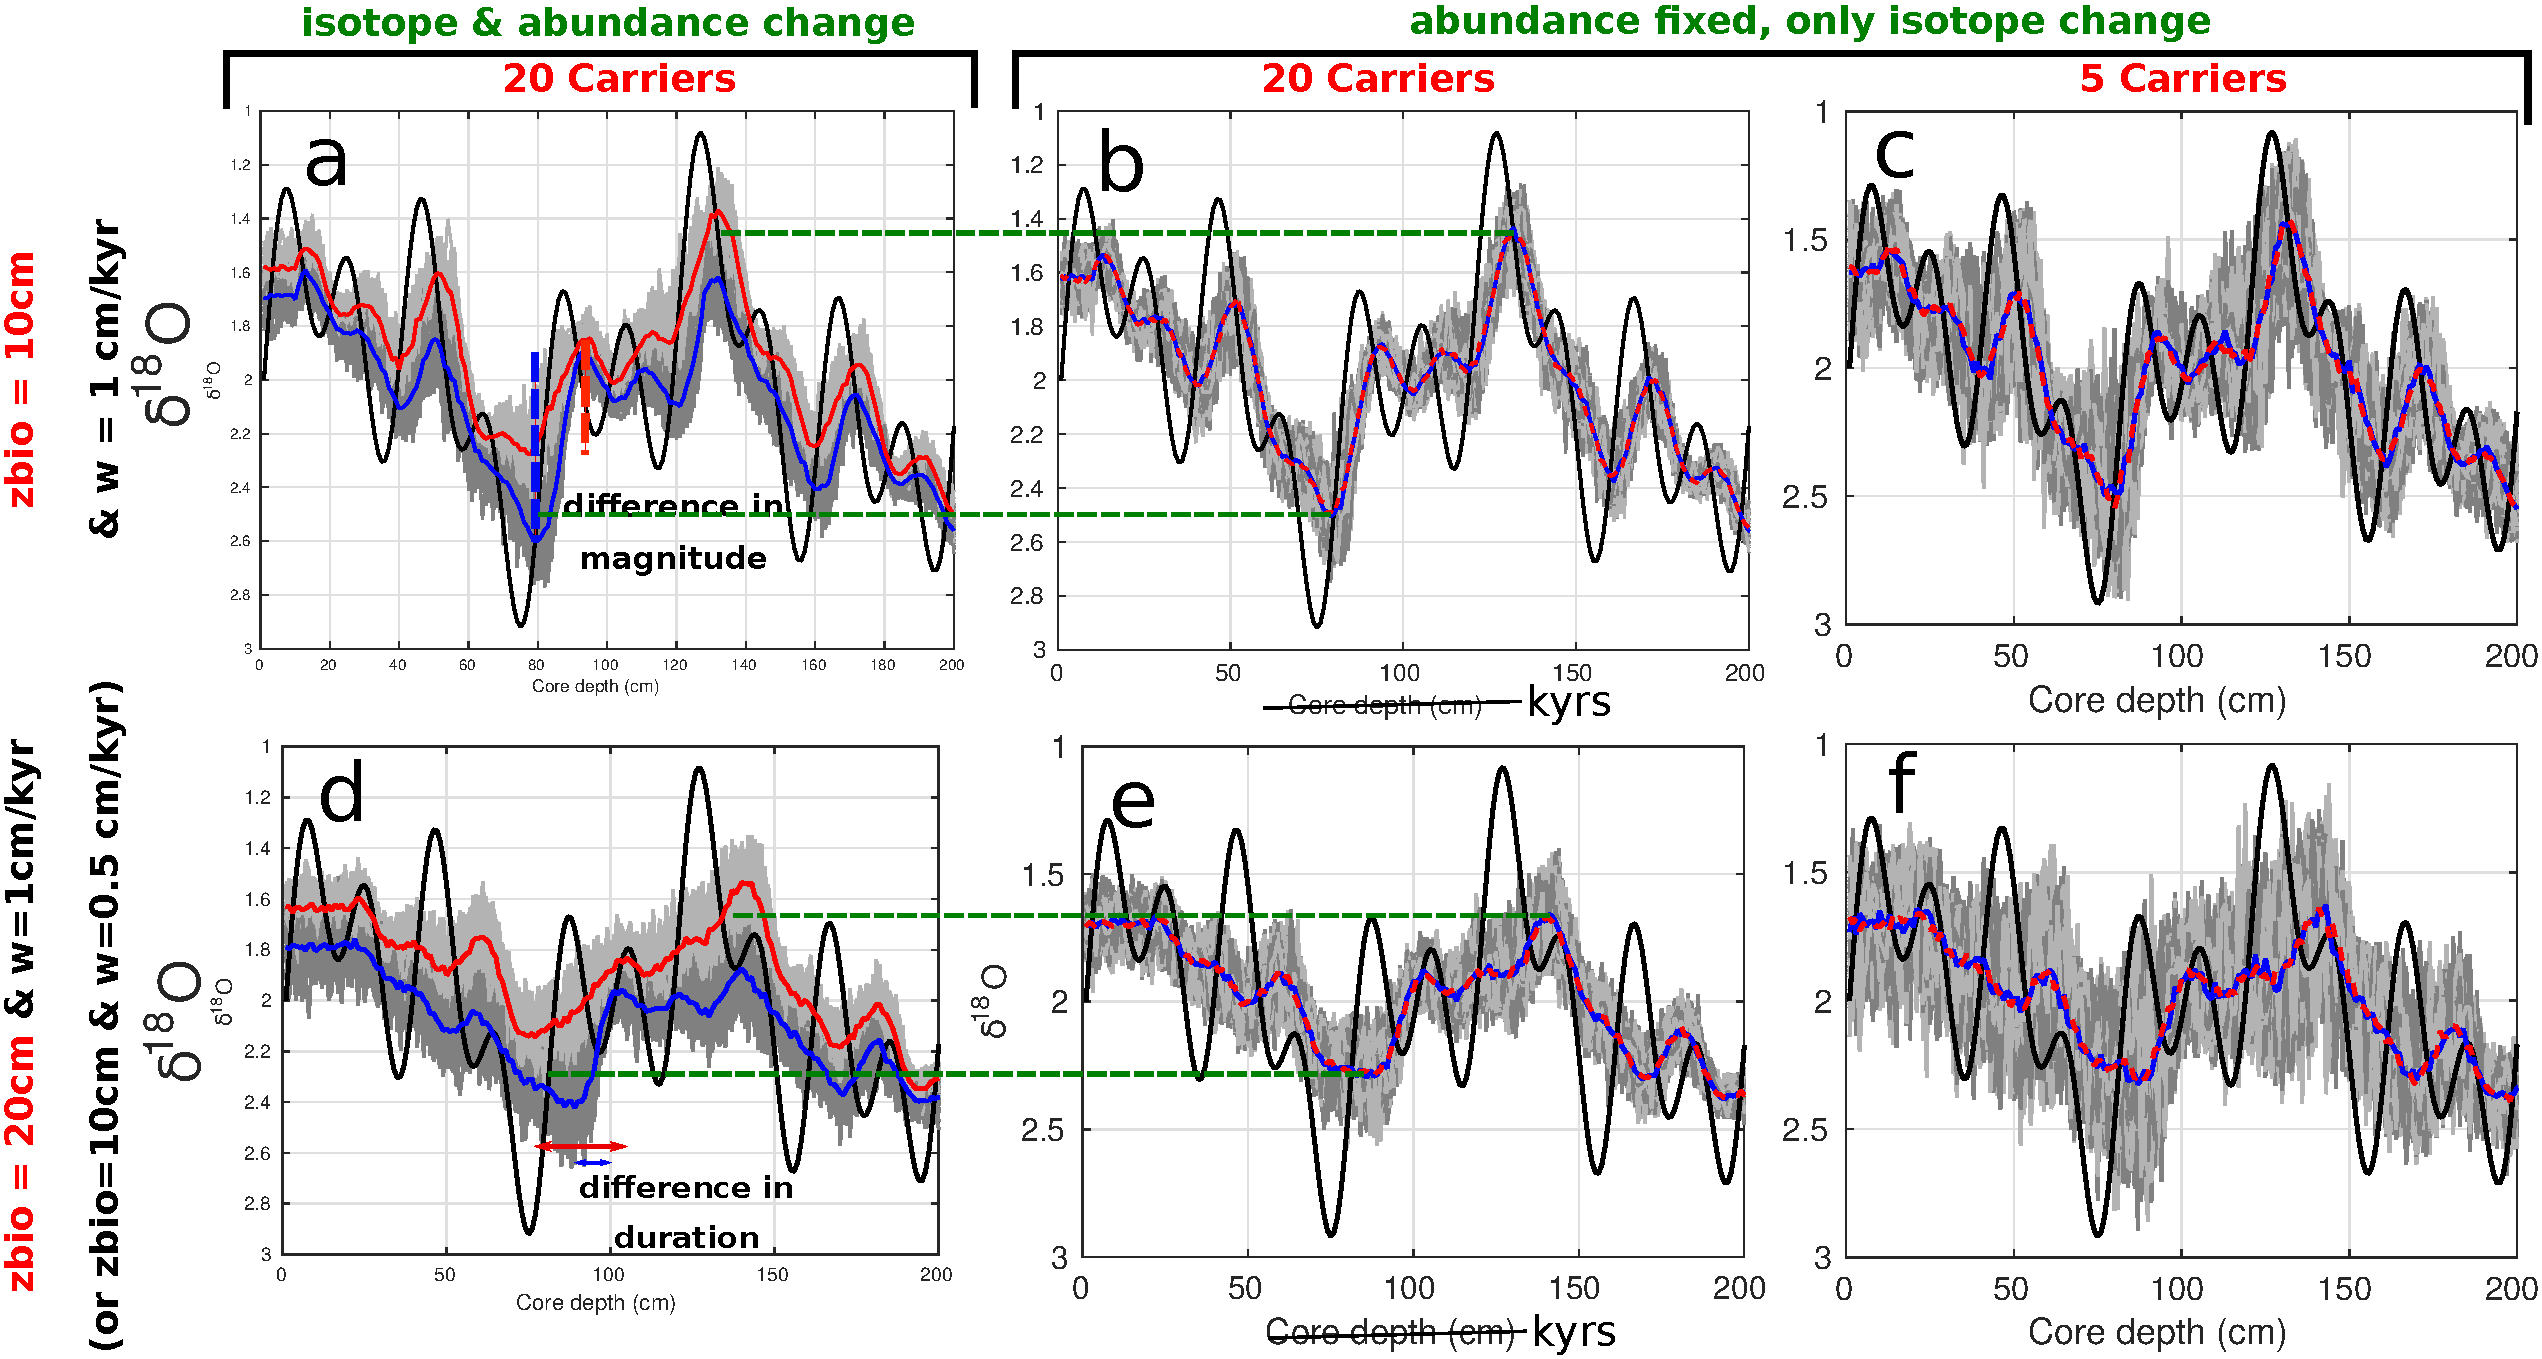
\includegraphics[width=0.9\textwidth]{figures/JustABU_3ycles_combined.pdf}%\caption{Observations from}
\end{figure}
\end{frame}

\begin{frame}
\frametitle{Example: 3 cycles + point events}
\begin{figure}[hbtp]
\hspace*{-0.8cm}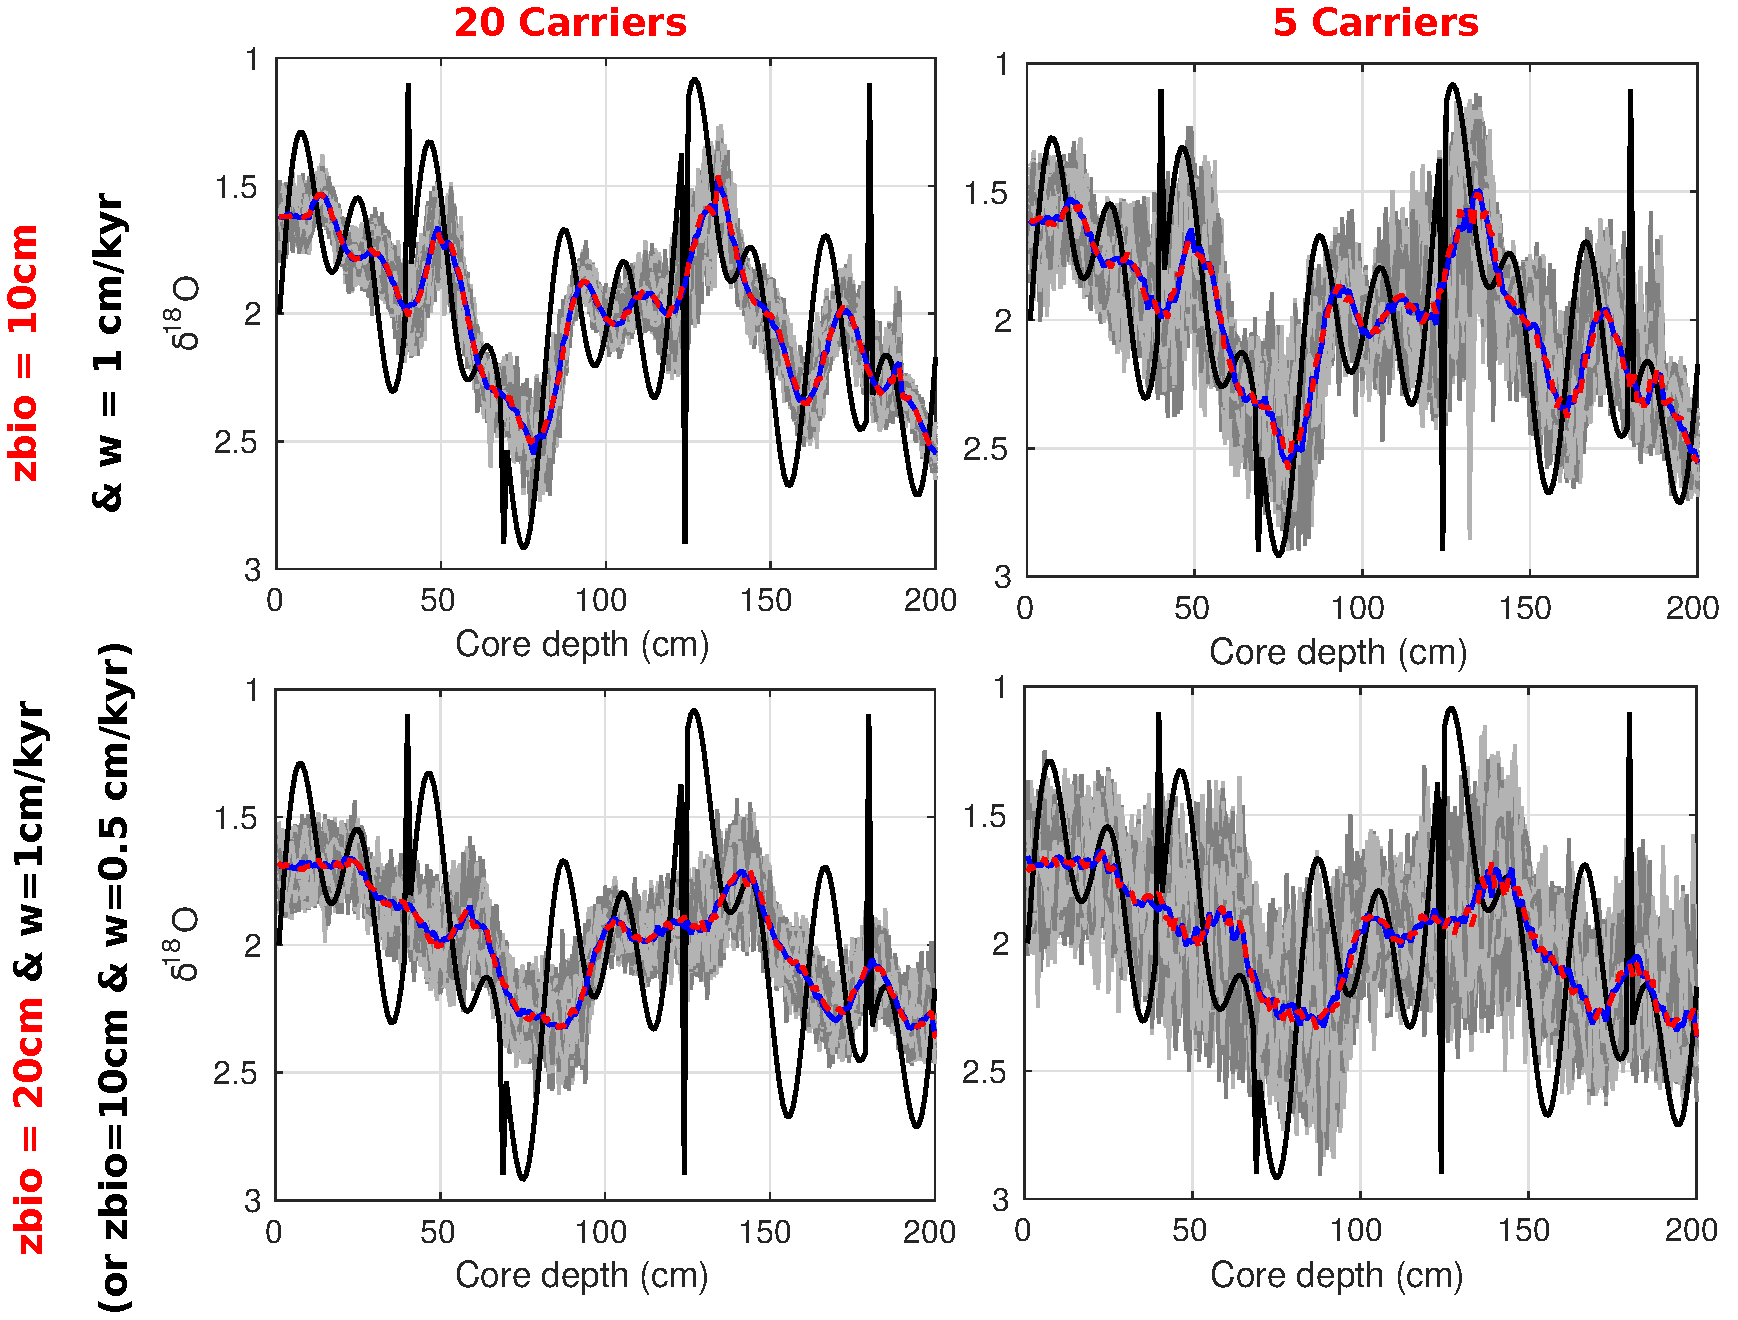
\includegraphics[width=0.9\textwidth]{figures/JustABU_3ycles_combined_pointevents.pdf}%\caption{Observations from}
\end{figure}
\end{frame}

\begin{frame}
\frametitle{Example: 3 cycles + step changes}
\begin{figure}[hbtp]
\hspace*{-0.8cm}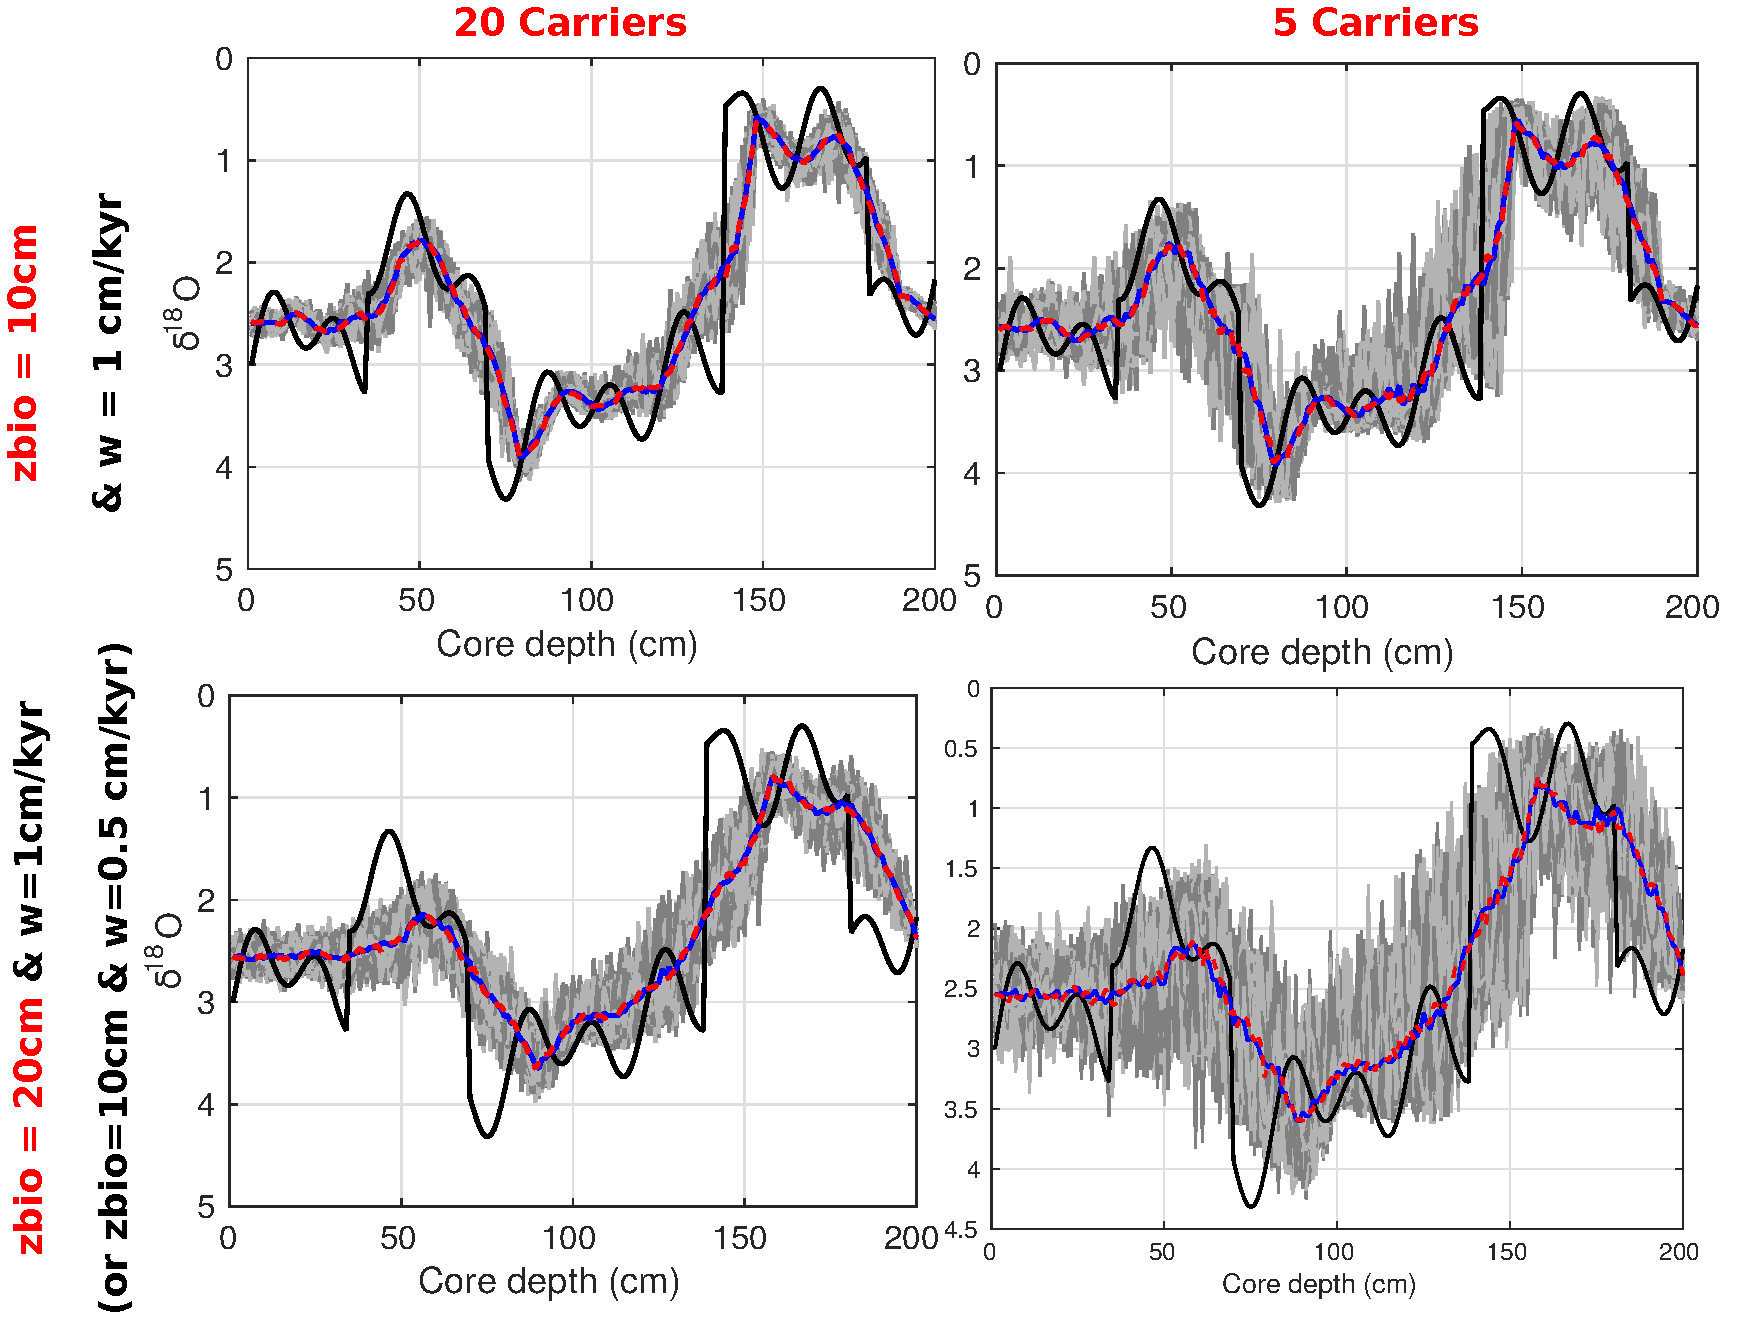
\includegraphics[width=0.9\textwidth]{figures/JustABU_3ycles_combined_gradual.pdf}%\caption{Observations from}
\end{figure}
\end{frame}


\end{document}


